%%%%%%%%%%%%%%%%%%%%%%%%%%%%%%%%%%%%%%%%%%%%%%%%%%%%%%%%%%%%%%%%%%%%%%
% How to use writeLaTeX: 
%
% You edit the source code here on the left, and the preview on the
% right shows you the result within a few seconds.
%
% Bookmark this page and share the URL with your co-authors. They can
% edit at the same time!
%
% You can upload figures, bibliographies, custom classes and
% styles using the files menu.
%
% If you're new to LaTeX, the wikibook is a great place to start:
% http://en.wikibooks.org/wiki/LaTeX
%
%%%%%%%%%%%%%%%%%%%%%%%%%%%%%%%%%%%%%%%%%%%%%%%%%%%%%%%%%%%%%%%%%%%%%%
\documentclass{tufte-book}

\hypersetup{colorlinks}% uncomment this line if you prefer colored hyperlinks (e.g., for onscreen viewing)

%%
% Book metadata
%\title{A Tufte-Style Book\thanks{Thanks to Edward R.~Tufte for his inspiration.}}
%\author[The Tufte-LaTeX Developers]{The Tufte-LaTeX\ Developers}
%\publisher{Publisher of This Book}
\usepackage[spanish, es-tabla]{babel}
\usepackage[utf8x]{inputenc}
\usepackage[T1]{fontenc}
\usepackage{chemfig}

\title{Qu\'imica F\'isica II}
%%
% If they're installed, use Bergamo and Chantilly from www.fontsite.com.
% They're clones of Bembo and Gill Sans, respectively.
%\IfFileExists{bergamo.sty}{\usepackage[osf]{bergamo}}{}% Bembo
%\IfFileExists{chantill.sty}{\usepackage{chantill}}{}% Gill Sans

\usepackage{microtype}

%%
% For nicely typeset tabular material
\usepackage{booktabs}

%%
% For graphics / images
\usepackage{graphicx}
\setkeys{Gin}{width=\linewidth,totalheight=\textheight,keepaspectratio}
\graphicspath{{graphics/}}

% The fancyvrb package lets us customize the formatting of verbatim
% environments.  We use a slightly smaller font.
\usepackage{fancyvrb}
\fvset{fontsize=\normalsize}

%%
% Prints argument within hanging parentheses (i.e., parentheses that take
% up no horizontal space).  Useful in tabular environments.
\newcommand{\hangp}[1]{\makebox[0pt][r]{(}#1\makebox[0pt][l]{)}}

%%
% Prints an asterisk that takes up no horizontal space.
% Useful in tabular environments.
\newcommand{\hangstar}{\makebox[0pt][l]{*}}

%%
% Prints a trailing space in a smart way.
\usepackage{xspace}


\setcounter{secnumdepth}{0}

% Allows for fancy math alignments
\usepackage{amsmath}
\usepackage{bm}
%\numberwithin{equation}{chapter}
%%

% Theorems
\newtheorem{theorem}{Postulado}
 
% Prints the month name (e.g., January) and the year (e.g., 2008)
\newcommand{\monthyear}{%
  \ifcase\month\or January\or February\or March\or April\or May\or June\or
  July\or August\or September\or October\or November\or
  December\fi\space\number\year
}

% Prints an epigraph and speaker in sans serif, all-caps type.
\newcommand{\openepigraph}[2]{%
  %\sffamily\fontsize{14}{16}\selectfont
  \begin{fullwidth}
  \sffamily\large
  \begin{doublespace}
  \noindent\allcaps{#1}\\% epigraph
  \noindent\allcaps{#2}% author
  \end{doublespace}
  \end{fullwidth}
}

% Inserts a blank page
\newcommand{\blankpage}{\newpage\hbox{}\thispagestyle{empty}\newpage}

\usepackage{units}
\usepackage{amssymb}
\usepackage{mathabx}
\usepackage{braket}

\usepackage{csquotes}

% Typesets the font size, leading, and measure in the form of 10/12x26 pc.
\newcommand{\measure}[3]{#1/#2$\times$\unit[#3]{pc}}

% Macros for typesetting the documentation
\newcommand{\hlred}[1]{\textcolor{Maroon}{#1}}% prints in red
\newcommand{\hangleft}[1]{\makebox[0pt][r]{#1}}
\newcommand{\hairsp}{\hspace{1pt}}% hair space
\newcommand{\hquad}{\hskip0.5em\relax}% half quad space
\newcommand{\TODO}{\textcolor{red}{\bf TODO!}\xspace}
\newcommand{\ie}{\textit{i.\hairsp{}e.}\xspace}
\newcommand{\eg}{\textit{e.\hairsp{}g.}\xspace}
\newcommand{\na}{\quad--}% used in tables for N/A cells
\providecommand{\XeLaTeX}{X\lower.5ex\hbox{\kern-0.15em\reflectbox{E}}\kern-0.1em\LaTeX}
\newcommand{\tXeLaTeX}{\XeLaTeX\index{XeLaTeX@\protect\XeLaTeX}}
% \index{\texttt{\textbackslash xyz}@\hangleft{\texttt{\textbackslash}}\texttt{xyz}}
\newcommand{\tuftebs}{\symbol{'134}}% a backslash in tt type in OT1/T1
\newcommand{\doccmdnoindex}[2][]{\texttt{\tuftebs#2}}% command name -- adds backslash automatically (and doesn't add cmd to the index)
\newcommand{\doccmddef}[2][]{%
  \hlred{\texttt{\tuftebs#2}}\label{cmd:#2}%
  \ifthenelse{\isempty{#1}}%
    {% add the command to the index
      \index{#2 command@\protect\hangleft{\texttt{\tuftebs}}\texttt{#2}}% command name
    }%
    {% add the command and package to the index
      \index{#2 command@\protect\hangleft{\texttt{\tuftebs}}\texttt{#2} (\texttt{#1} package)}% command name
      \index{#1 package@\texttt{#1} package}\index{packages!#1@\texttt{#1}}% package name
    }%
}% command name -- adds backslash automatically
\newcommand{\doccmd}[2][]{%
  \texttt{\tuftebs#2}%
  \ifthenelse{\isempty{#1}}%
    {% add the command to the index
      \index{#2 command@\protect\hangleft{\texttt{\tuftebs}}\texttt{#2}}% command name
    }%
    {% add the command and package to the index
      \index{#2 command@\protect\hangleft{\texttt{\tuftebs}}\texttt{#2} (\texttt{#1} package)}% command name
      \index{#1 package@\texttt{#1} package}\index{packages!#1@\texttt{#1}}% package name
    }%
}% command name -- adds backslash automatically
\newcommand{\docopt}[1]{\ensuremath{\langle}\textrm{\textit{#1}}\ensuremath{\rangle}}% optional command argument
\newcommand{\docarg}[1]{\textrm{\textit{#1}}}% (required) command argument
\newenvironment{docspec}{\begin{quotation}\ttfamily\parskip0pt\parindent0pt\ignorespaces}{\end{quotation}}% command specification environment
\newcommand{\docenv}[1]{\texttt{#1}\index{#1 environment@\texttt{#1} environment}\index{environments!#1@\texttt{#1}}}% environment name
\newcommand{\docenvdef}[1]{\hlred{\texttt{#1}}\label{env:#1}\index{#1 environment@\texttt{#1} environment}\index{environments!#1@\texttt{#1}}}% environment name
\newcommand{\docpkg}[1]{\texttt{#1}\index{#1 package@\texttt{#1} package}\index{packages!#1@\texttt{#1}}}% package name
\newcommand{\doccls}[1]{\texttt{#1}}% document class name
\newcommand{\docclsopt}[1]{\texttt{#1}\index{#1 class option@\texttt{#1} class option}\index{class options!#1@\texttt{#1}}}% document class option name
\newcommand{\docclsoptdef}[1]{\hlred{\texttt{#1}}\label{clsopt:#1}\index{#1 class option@\texttt{#1} class option}\index{class options!#1@\texttt{#1}}}% document class option name defined
\newcommand{\docmsg}[2]{\bigskip\begin{fullwidth}\noindent\ttfamily#1\end{fullwidth}\medskip\par\noindent#2}
\newcommand{\docfilehook}[2]{\texttt{#1}\index{file hooks!#2}\index{#1@\texttt{#1}}}
\newcommand{\doccounter}[1]{\texttt{#1}\index{#1 counter@\texttt{#1} counter}}

% Generates the index
\usepackage{makeidx}
\makeindex

\begin{document}

% Front matter
%\frontmatter

% r.1 blank page
%\blankpage

%% v.2 epigraphs
%\newpage\thispagestyle{empty}
%\openepigraph{%
%The public is more familiar with bad design than good design.
%It is, in effect, conditioned to prefer bad design, 
%because that is what it lives with. 
%The new becomes threatening, the old reassuring.
%}{Paul Rand%, {\itshape Design, Form, and Chaos}
%}
%\vfill
%\openepigraph{%
%A designer knows that he has achieved perfection 
%not when there is nothing left to add, 
%but when there is nothing left to take away.
%}{Antoine de Saint-Exup\'{e}ry}
%\vfill
%\openepigraph{%
%\ldots the designer of a new system must not only be the implementor and the first 
%large-scale user; the designer should also write the first user manual\ldots 
%If I had not participated fully in all these activities, 
%literally hundreds of improvements would never have been made, 
%because I would never have thought of them or perceived 
%why they were important.
%}{Donald E. Knuth}
%



% r.3 full title page
\maketitle


%% v.4 copyright page
%\newpage
%\begin{fullwidth}
%~\vfill
%\thispagestyle{empty}
%\setlength{\parindent}{0pt}
%\setlength{\parskip}{\baselineskip}
%Copyright \copyright\ \the\year\ \thanklessauthor
%
%\par\smallcaps{Published by \thanklesspublisher}
%
%\par\smallcaps{tufte-latex.googlecode.com}
%
%\par Licensed under the Apache License, Version 2.0 (the ``License''); you may not
%use this file except in compliance with the License. You may obtain a copy
%of the License at \url{http://www.apache.org/licenses/LICENSE-2.0}. Unless
%required by applicable law or agreed to in writing, software distributed
%under the License is distributed on an \smallcaps{``AS IS'' BASIS, WITHOUT
%WARRANTIES OR CONDITIONS OF ANY KIND}, either express or implied. See the
%License for the specific language governing permissions and limitations
%under the License.\index{license}
%
%\par\textit{First printing, \monthyear}
%\end{fullwidth}

% r.5 contents
%\tableofcontents
%\listoffigures
%\listoftables

%% r.7 dedication
%\cleardoublepage
%\vfill
%\begin{doublespace}
%\noindent\fontsize{18}{22}\selectfont\itshape
%\nohyphenation
%Dedicated to those who appreciate \LaTeX{} 
%and the work of \mbox{Edward R.~Tufte} 
%and \mbox{Donald E.~Knuth}.
%\end{doublespace}
%\vfill
%\vfill


\chapter{Antecedentes de la Mecánica Cuántica}
A finales del s. XIX se producen una serie de cambios muy 
importantes  en la Física debido, en primer término, a una
serie de observaciones experimentales que la Física Clásica
no era capaz de explicar.

\section{Radiación del Cuerpo Negro}
La primera de estas limitaciones parte de un fenómeno que 
podemos observar cotidianamente. Cuando calentamos un metal 
a muy elevadas temperaturas vemos que empieza a cambiar de 
color, adquiriendo tonalidades primero rojizas y luego azuladas.
Esto se debe a que  el cuerpo calentado emite una radiación
electromagnética. No todas las frecuencias están igualmente 
presentes en la radiación. Si estudiamos cómo cambia la distribución
de longitudes de onda, $\lambda$,  a medida que va aumentando
la temperatura, veremos que el máximo de la distribución se 
desplaza hacia longitudes de onda más bajas. Esta observación la
captura la \textbf{ley de desplazamiento de Wien},
\begin{equation}
\lambda_\mathrm{max}T=\mathrm{constante}.
\label{eq:Wien}
\end{equation}

Definimos el \textbf{cuerpo negro} como un objeto que es capaz de 
absorber todas las longitudes de onda uniformemente. Podemos pensar
en él como un dispositivo experimental con una cavidad reflectante
en el interior, que se prepara en equilibrio a una temperatura $T$,
y en el que hay apenas un pequeño orificio, que nos permite medir 
la radiación. \textbf{Lord Rayleigh} trató este problema de manera
clásica, asumiendo que el campo electromagnético se podía describir
como una colección de osciladores con todas las frecuencias o
longitudes de onda posibles. Si había una radiación de una longitud
de onda determinada, esta radiación se correspondería con un oscilador
excitado. A partir de una descripción que asumía que la temperatura
distribuiría su energía de acuerdo con el \textbf{principio de
equipartición de la energía}, llegó con la ayuda de \textbf{James
Jeans} a la siguiente relación:
\begin{equation}
\rho=\frac{8\pi k_BT}{\lambda^4}
\label{eq:rayleigh-jeans}
\end{equation}
Esta ecuación, conocida como la \textbf{ecuación de Rayleigh-Jeans},
expresa la contribución a la energía de la radiación para cada una de las 
longitudes de onda $\lambda$, o la densidad de estados, $\rho$. 
Como vemos la dependencia con  $\lambda$ es inversa con la
cuarta potencia.  A valores elevados de $\lambda$, la predicción
es acertada, pero a valores bajos, correspondiente a radiación
de muy alta energía, la densidad aumentaría monotónicamente. 
Esto  conduciría a la denominada ``catástrofe 
ultravioleta'', porque de acuerdo con este crecimiento monotónico
la densidad nunca dejaría de aumentar. Este resultado revelaba un
fallo en la descripción clásica del sistema.

\textbf{Max Planck} pudo resolver este problema asumiendo que la
energía
de cada oscilador estaba limitada a una serie de valores discretos,
es decir, estaba cuantizada. La energía de cada oscilador de 
frecuencia $\nu$ debía ser un múltiplo entero de la cantidad
$h\nu$. Es decir, 
\begin{equation}
E=nh\nu
\end{equation}
donde $n=1,2,3...$. De esta manera la expresión resultante
para la densidad de estados era la denominada \textbf{distribución
de Planck},
\begin{equation}
    \rho=\frac{8\pi h c}{\lambda^5(\mathrm{e}^{hc/\lambda k_BT}-1)}\
\label{eq:planck}
\end{equation}
En la teoría de Planck, la constante $h$ era indeterminada,
pero ajustando a los datos experimentales se pudo recuperar 
su valor de $h=6.626\times 10^{-34}$J$\cdot$s. De acuerdo con
esta nueva interpretación ``cuántica'', los osciladores se 
excitan sólo cuando hay suficiente energía disponible para 
alcanzar la energía $h\nu$.

\section{El Efecto Fotoeléctrico}
La segunda evidencia experimental que iba más allá de lo que la 
Física clásica era capaz de predecir es el denominado efecto
fotoeléctrico. El efecto fotoeléctrico indica que los fotones
se comportan como partículas que son capaces de colisionar
con otras partículas. 
En este caso, el experimento consistía en 
exponer a un material determinado a una radiación ultravioleta.
Hasta alcanzar una determinada frecuencia de radiación, $\nu_0$, 
no se observaba nada. Pero a partir de $\nu_0$ empezaban a 
liberarse electrones. La frecuencia $\nu_0$ era además 
característica de cada material.

Otro aspecto
interesante a resaltar de este proceso de ionización es que la
energía cinética de esos electrones dependía de la frecuencia
de la radiación incidente, y era independiente de la intensidad
de esta radiación, lo cual era contrario a las predicciones de
Maxwell. Incluso con muy bajas intensidades de radiación
se producía la ionización del material con tal de que se cumpliese
la condici\'on $\nu>\nu_0$.

¿De qué manera se resolvió este problema? Ya en el s. XX, 
\textbf{Albert Einstein} propuso una solución a esta paradoja,
el mismo año en que describió el movimiento Browniano y la 
Teoría de la Relatividad. Para liberar un electrón, teorizó, es
necesario un \textbf{cuanto de energía} superior a un umbral $\nu_0$, y la
energía excedente se libera en forma de energía cinética con la
que sale despedido el electrón. Así define la llamada \textbf{"work
function"},
\begin{equation}
\frac{1}{2}m_ev^2=h\nu - \Phi
\end{equation}
donde $h\nu$ es la energía de la radiación incidente, $\Phi$ es
el umbral necesario para producir la emisión del electrón y
en la lado izquierdo de la ecuación nos encontramos con la 
expresión familiar de la energía cinética. En el caso de que
$h\nu<\Phi$ no se produce liberación de electrones, pero si
por el contrario $h\nu>\Phi$ entonces sí que se produce
ionización y con una cantidad de energía que podemos calcular.

\section{Hipótesis de de Broglie}
De modo que ya hemos establecido el carácter de partícula de las
ondas. Experimentos similares sirvieron para establecer
el comportamiento como onda de los electrones. El experimento
crucial lo realizaron \textbf{Davisson} y \textbf{Germer}, 
que observaron la difracción de electrones en un cristal. 
La difracción es la interferencia causada por un objeto 
interpuesto en el camino de una onda, y al hacer este experimento
se observó que también los electrones, comportándose como ondas,
difractaban.

Otras partículas también son capaces de difractar, como han 
revelado después experimentos en partículas $\alpha$ o en
el hidrógeno molecular, confirmando que las partículas tienen
características de ondas. 

¿Pero cómo racionalizamos esta dualidad de ondas y cuerpos?
Una primera indicación nos la da la relación del físico Francés
\textbf{Louis de Broglie}, que propuso que una partícula que viajase
con un momento lineal $p$ tendría una longitud de onda asociada
\begin{equation}
\lambda=\frac{h}{p}\label{eq:debroglie}
\end{equation}
Los cuerpos de gran tamaño tienen momentos lineales enormes, debido
a su gran masa. Por eso sus longitudes de onda son indetectables
y las propiedades oscilatorias de los cuerpos macroscópicos no 
pueden ser observados.	

\section{Principio de Incertidumbre de Heisenberg}
Otra de las grandes rupturas que establece la Mecánica Cuántica 
con la Mecánica Clásica es nuestra capacidad de medir una 
determinada propiedad con precisión arbitraria. Dentro de la 
formulación de la Mecánica Cuántica es muy importante el Principio
de Incertidumbre, enunciado por \textbf{Werner Heisenberg} en 1927
y que le valió un Premio Nobel en 1932 por "la creación de la Mecánica
Cuántica". 
Establece que es imposible determinar simultáneamente el momento 
y la posición de una partícula. 

Aunque veremos este principio en 
mayor profundidad más adelante en el curso, la precisión de una
medida viene determinada por
\begin{equation}
    \Delta x\Delta q\geq 1/2\hbar\label{eq:heiss}
\end{equation}
donde $\Delta p=(\langle p^2\rangle-\langle p \rangle^2)^{1/2}$ y
$\Delta q=(\langle q^2\rangle-\langle q\rangle^2)^{1/2}$. En realidad
el principio de incertidumbre no sólo afecta al momento y a la posición, sino a 
cualquier par de \textbf{variables complementarias}. Del mismo modo
que en la Ecuación \ref{eq:heiss} para posición y momento, para 
la duración de un proceso cuántico $t$ y su energía $E$ podemos
escribir
\begin{equation}
    \Delta E\Delta t\geq 1/2\hbar.
\end{equation}

\section{Espectros atómicos}
La última evidencia experimental que comentaremos procede de los 
espectros atómicos. Si nosotros obtenemos un espectro de emisión
de un elemento como el hidrógeno, con lo que nos encontramos
es que el espectro es discontinuo. Por tanto, la emisión de un
átomo se produce sólo a unos determinados valores de la longitud
de onda. De paso podemos decir que en el caso de una molécula 
también el espectro de absorción, que corresponde a frecuencias
que permiten a una molécula cambiar de estado, es discontinuo.

Esto hizo que tuvieran que reformularse los modelos atómicos que 
se empleaban, y que parecían incompatibles con esta discontinuidad.
El primer modelo que tuvo en consideración esta propiedad fue
el de \textbf{Niels Bohr}, que partía de dos suposiciones: 
\begin{itemize}[i]
    \item La primera es que un electrón orbita alrededor del
    núcleo en un conjunto discreto de estados estacionarios, 
    correspondientes a órbitas circulares que satisfacen que la
    fuerza centrífuga y la atracción entre el núcleo y el electrón
    son iguales.
    \begin{equation}
        \frac{e^2}{4\pi \epsilon_0 r^2}=m_e\frac{v^2}{r}
    \end{equation}
    \item La segunda suposición era la que introducía la cuantización
    y asumía que las órbitas permitidas debían satisfacer la relación
    $L=n\hbar=m_evr$, donde $L$ es una magnitud denominada ``acción''.
\end{itemize}
Reorganizando estas ecuaciones podemos calcular el radio de las órbitas,
\begin{equation}
    r_n=\bigg(\frac{4\pi \epsilon_0\hbar^2}{m_ee^2}\bigg)n^2=a_0n^2    
\end{equation}
y la correspondiente energía de los diferentes niveles
\begin{equation}
    \begin{split}
%    A & = \frac{\pi r^2}{2} \\
% & = \frac{1}{2} \pi r^2
    E_n= & \frac{1}{2}m_ev^2 - \frac{1}{4\pi \epsilon_0}\frac{e^2}{r}=\\
    & -\frac{m_e}{2\hbar^2}\bigg(\frac{e^2}{4\pi\epsilon_0}\bigg)\bigg(\frac{1}{n^2}\bigg)
    \end{split}
\end{equation}
Para el hidrógeno, esta descripción es satisfactoria, y fue capaz de
explicar transiciones entre niveles de acuerdo con la siguiente 
expresión
\begin{equation}
    \tilde{\nu}=R_H\bigg(\frac{1}{n^2_1} -\frac{1}{n^2_2}\bigg) 
    \label{eq:Rydberg}
\end{equation}
donde $\tilde{\nu}=1/\lambda$ es el número de onda, $R_H$=109677 cm$^{-1}$ 
es la constante de Rydberg del átomo de hidrógeno. La Ecuación 
\ref{eq:Rydberg} explica las líneas espectrales de Lyman, Balmer, 
y Paschen, donde $n_1=1,2, 3$ y $n_2=2,3,4$, respectivamente.

\chapter{Postulados de la Mecánica Cuántica}
La Mecánica Cuántica está basada en una serie de
postulados. Los postulados son, según el diccionario
de la Real Academia de la Lengua, proposiciones cuya
verdad se admite sin pruebas y que sirven de base para
ulteriores razonamientos. A continuación introduciremos
los postulados de la Mecánica Cuántica, que usaremos 
como fundamento para describir más adelante sistemas
sencillos.

\section*{Estados y funciones de onda}
\begin{theorem}
Todas las propiedades observables de un sistema físico 
están contenidas en su función de onda, $\psi(q,t)$,
dependiente de las coordenadas ($q$) de las
partículas que componen el sistema y del tiempo ($t$). 
\end{theorem}

En Mecánica Cuántica, por tanto, el concepto de 
trayectoria es remplazado por la \textbf{función de
onda}, que contiene toda la información dinámica 
sobre el sistema.

\section{Interpretación de la función de onda}
Para desarrollar una intuición sobre el significado
de la función de onda es útil recurrir a la 
denominada \textbf{interpretación de 
Born}, que también enunciamos en la forma de 
postulado.
\begin{theorem} 
La probabilidad de que una partícula se encuentre en 
un volumen $\tau$ en el punto $r$ es proporcional
a $|\psi(r)|^2d\tau=\psi^\star \psi d\tau$
\end{theorem}
El cuadrado de la función de onda es por tanto una
\textbf{densidad de probabilidad}. Y si tomamos la
integral de esta densidad en una pequeña region 
$d\tau$ del espacio, obtendremos la probabilidad de
encontrar el sistema en esa región $d\tau$. En la 
medida en que la suma de todas las probabilidades
debe ser igual a la unidad, la función de onda debe 
cumplir una condición de normalización,
\begin{equation}
    N^2\int_{-\infty}^\infty\psi^\star\psi dx=1
    \label{eq:norm}
\end{equation}

En ocasiones, para el caso tridimensional, puede 
ser más conveniente escribir esta condición de 
normalización en coordenadas esféricas, es decir,
en función del radio $r$, la colatitud $\theta$
y el ángulo azimutal $\phi$. La interconversión
entre coordenadas cartesianas y esféricas es 
trivial, 
\begin{equation}
  \begin{array}{@{}ll@{}}
    x = & r\sin\theta\cos\phi \\
    y = & r\sin\theta\sin\phi \\
    z = & \cos \theta
  \end{array}
\end{equation}
de tal manera que la integral normalizada que 
expresábamos en una sóla dimensión en la 
Ecuación~\ref{eq:norm} se puede reescribir usando
$d\tau=r^2\sin\theta drd\theta d\phi$ y modificando
los límites de integración de la siguiente manera
\begin{equation}
    \int_\infty^\infty\psi^\star\psi d\tau=
    \int_0^\infty\int_0^\pi\int_0^{2\pi}\psi^\star\psi r^2\sin\theta drd\theta d\phi
\end{equation}

La interpretación de Born y la ecuación de Schrödinger
que, como veremos más adelante, es una ecuación
diferencial de segundo orden, introducen una serie de
requisitos para las funciones de onda aceptables:
\begin{itemize}
    \item Debe ser unívoca, es decir, no debe 
    estar definida con más de un valor en cada punto.
    \item Debe tener un cuadrado integrable.
    \item Debe ser continua.
    \item Debe ser derivable.
\end{itemize}


\section{Observables y operadores}
\begin{theorem}
Los observables se representan mediante operadores 
Hermíticos.
\end{theorem}
Para entender este postulado debemos definir primero
los operadores. Los operadores, $\hat{\Omega}$, no son
sino funciones que convierten una función de onda 
en otra:
\begin{equation}
    \psi(q,t)\xrightarrow{\hat{\Omega}}\psi'(q,t)
\end{equation}
Un ejemplo de operador, pueden ser el operador
diferencial con respecto de $x$, $\hat{D}_x=\frac{d}{dx}$.
Al aplicarlo sobre la función \textit{seno}, obtenemos
la función \textit{coseno}.
\begin{equation}
    \hat{D}_x\sin x=\frac{d}{dx}\sin x =\cos x
\end{equation}
Un \textbf{operador lineal} es un tipo especial de operador
que satisface las siguientes relaciones
\begin{equation}
      \begin{array}{rl}
        \hat{\Omega}(\psi+\phi) &=\hat{\Omega}\psi + \hat{\Omega}\phi\\
        \hat{\Omega}c\psi &=c\hat{\Omega}\psi
    \end{array}
\end{equation}

Un tipo de operador particular en el que estamos 
interesados en Mecánica Cuántica son los que se pueden
expresar en la forma de una \textbf{ecuación de valores
propios}:
\begin{equation}
    \hat{\Omega}\psi(q,t)=\omega\psi(q,t)
\end{equation}
donde $\omega$ es el valor propio (\textit{eigenvalue})
correspondiente al operador $\hat{\Omega}$. Cuando
encontramos esta propiedad, entonces decimos que $\psi$ 
es función propia ($\textit{eigenfunction}$) de este
operador. Este tipo de expresión es la que nos vamos a
encontrar en el caso del operador Hamiltoniano, 
$\hat{H}$, para la energía total pero también para 
otros observables que mostramos en la 
Tabla~\ref{tab:operators}.

\begin{table}[h]
  \begin{center}
    %\footnotesize%
    \small
    \begin{tabular}{lcr}
      \toprule
      Nombre & Expresión \\
      \midrule
      Posición & $\hat{x}=x$ \\
      Momento lineal & $\hat{p}_x=-i\hbar \frac{\partial}{\partial x}$ \\
      Energía cinética & $\hat{K}=\frac{\hat{p}_x^2}{2m}=
      -\frac{\hbar^2}{2m}\frac{\partial^2}{\partial x^2}$\\
      Energía potencial & $\hat{V}=V(x,y,z)$ \\
      Hamiltoniano & $\hat{H}=\hat{K}+\hat{V}$ \\
      \bottomrule
    \end{tabular}
  \end{center}
  \caption{Operadores habituales en Mecánica Cuántica.}
  \label{tab:operators}
\end{table}

Finalmente, un \textbf{operador hermítico} es el que
satisface la siguiente relación
\begin{equation}
    \int\psi_i^\star\hat{\Omega}\psi_jdx=
    \bigg\{\int\psi_j^\star\hat{\Omega}\psi_idx\bigg\}^\star
\end{equation}
Estos operadores tienen dos propiedades especiales:
\begin{itemize}
    \item Sus valores propios son reales.
    \item Sus funciones propias son ortogonales, es decir:
    $\int_{-\infty}^\infty\psi_1^\star\psi_2d\tau=0$
\end{itemize}
El conjunto de funciones propias de un operador 
    hermítico forman un \textbf{conjunto completo}.

\section{El resultado de una medida}
\begin{theorem}
Cuando un sistema está descrito por una función de onda
$\psi$, el valor del observable $\Omega$ en una serie 
de medidas es igual al valor promedio (“expectation 
value”) del operador.
\end{theorem}
Cuando nos encontramos con que una función de onda no es
función propia de un operador $\hat{\Omega}$ no podemos
utilizar el método de los operadores para obtener el valor
promedio de $\Omega$. Sin embargo podemos expresar la
función de onda como una combinación lineal o
\textbf{superposición} de un conjunto de funciones
propias
\begin{equation}
\psi =  c_1\psi_1 + c_2\psi_2 + ... = \sum_kc_k\psi_k    
\end{equation}
En esta expresión los valores de $c_k$ son coeficientes
reales o imaginarios y las funciones de onda $\psi_k$
corresponden con diferentes estados del sistema. Esto
significa que cualquier función de onda puede 
expresarse como una combinación lineal de estos estados.

Cuando se realiza una medida, se obtendrá el valor 
propio $\omega_k$ correspondiente a una de las funciones
propias $\psi_k$ del operador. La probabilidad de
encontrar cada una de las soluciones es proporcional
al cuadrado del módulo  del coeficiente $|c_k|^2$ dentro
de la combinación lineal. El promedio tras un gran número
de observaciones lo da el valor esperado, $\langle
\Omega\rangle$.



\section{La ecuación de Schrödinger}
\begin{theorem}
La función de onda evoluciona en el tiempo de acuerdo 
con la ecuación de Schrödinger dependiente del tiempo:
\begin{equation}
    \hat{H}\Psi = i\hbar\frac{\partial \Psi}{\partial t}
\end{equation}
\end{theorem}
Como conocemos el operador hamiltoniano, $\hat{H}$ (ver
Tabla \ref{tab:operators}), podemos escribir si trabajamos
en una sola dimensión
\begin{equation}
    \hat{H}\Psi = 
      -\frac{\hbar^2}{2m}\frac{\partial^2}{\partial x^2}\Psi + V(x)\Psi = i\hbar\frac{\partial \Psi}{\partial t}
\end{equation}
En el caso de los estados estacionarios 
se puede separar la parte de la función de onda
que depende de las coordenadas de la parte que 
depende del tiempo,
\begin{equation}
    \Psi(q,t)=\psi(q)\tau(t)
\end{equation}
Al aplicar el operador hamiltoniano 
sobre este tipo de función de onda
aquel afecta únicamente a la parte
que depende de las coordenadas. Por
tanto,
\begin{equation}
    \hat{H}\Psi(q,t)=
    \tau(t)\hat{H}\psi(q)=
    i\hbar\frac{\partial\psi(q)\tau(t)}{\partial t}=
    i\hbar\psi(q)\frac{\partial \tau(t)}{\partial t}
\end{equation}
Reorganizando los términos en esta ecuación encontramos
lo siguiente
\begin{equation}
    \frac{1}{\psi(q)}\hat{H}\psi(q) = \frac{i\hbar}{\tau(t)}\frac{\partial \tau(t)}{\partial t}= E
    \label{eq:schro-2}
\end{equation}
A partir de los dos términos a la derecha de la Ecuación
\ref{eq:schro-2} podemos encontrar la solución para la
Ecuación de Schrödinger,
\begin{equation}
    \tau(t)=A\exp(-iEt/\hbar)
\end{equation}
Por tanto la función de onda para un estado estacionario
es
\begin{equation}
    \Psi(q,t)=\psi(q)\exp(-iEt/\hbar)
\end{equation}
Si obtenemos $\Psi(q,t)^2$ veremos que las funciones para un
estado estacionario tienen una energía definida 
y una densidad de probabilidad constante en el tiempo.
En un estado estacionario podemos medir todos y cada uno de los 
operadores que conmuten con el hamiltoniano. Estos son el 
equivalente de las constantes de movimiento de la mecánica clásica.

\section{El principio de incertidumbre}
Ahora que entendemos más a fondo el funcionamiento de los
operadores podemos adentrarnos de nuevo en el
\textbf{Principio de Incertidumbre} enunciado por 
\textbf{Werner Heisenberg}. Como comentamos en el Tema 1
el principio establece en su formulación más básica que 
no se puede determinar con precisión  arbitraria el momento
y la posición de la partícula. 

Supongamos que tenemos una partícula perfectamente 
localizada en un punto del espacio. Utilizando el
principio de superposición, podemos obtener esta 
descripción combinando un gran número de ondas 
armónicas, es decir, generando un paquete de
ondas (\textit{wave packet}). Esto resultará en una
función de onda perfectamente localizada y por tanto
con un error muy pequeño en la posición ($\Delta x=0$).
Pero a su vez las distintas contribuciones a la función 
de onda tendrán muy diversos valores del momento lineal, 
lo que resulta en una gran incertidumbre en el valor 
del momento lineal ($\Delta p=\infty$). Si tenemos gran
certeza en uno de estos valores, entonces
tendremos gran incertidumbre en el otro valor.

El principio de incertidumbre, formulado típicamente para
$p$ y $q$, es en realidad más general. Si para cada 
operador $\hat{\Omega}$ podemos definir un error $\Delta\Omega$:
\begin{equation}
    (\Delta\Omega^2)=\sigma^2_\Omega=\langle (\hat{\Omega} - \langle \Omega\rangle)^2 \rangle=
    \langle\hat{\Omega}^2\rangle - \langle\Omega\rangle^2
\end{equation}
el principio de incertidumbre relaciona los errores de dos
\textbf{variables complementarias} de tal modo que
\begin{equation}
\Delta\Omega_1\Delta\Omega_2\geq
1/2|\langle[\Omega_1,\Omega_2]\rangle|
\end{equation}
donde  usamos el conmutador  $[\hat{\Omega}_1,\hat{\Omega}_2] =
\hat{\Omega}_1\hat{\Omega}_2 -\hat{\Omega}_2\hat{\Omega}_1$.
Son complementarias aquellas variables que no conmutan y para
las que se cumple 
$\hat{\Omega}_1(\hat{\Omega}_2\psi)\neq\hat{\Omega}_2(\hat{\Omega}_1\psi)$.
En el caso particular de la posición y el momento obtenemos que
\begin{equation}
    [\hat{x},\hat{p}_x] = i\hbar
\end{equation}
y por tanto son operadores
complementarios. Por el contrario, cuando
dos operadores hermíticos conmutan decimos 
que son \textbf{compatibles }, y comparten un conjunto
completo de funciones propias, $\psi_n$.

\section{Principio de exclusión o de Pauli}
Por último introduciremos una contribución decisiva
al desarrollo de la Mecánica Cuántica. El principio de
exclusión establece que las partículas cuánticas poseen una 
propiedad fundamental que toma un valor entero o semientero 
característico de cada partícula. Esta propiedad, 
llamada \textit{spin}, $s$, fue inicialmente introducida
por \textbf{Wolfgang Pauli} como lo que él denominaba una
dualidad no
describible clásicamente (``classically non-describable
two-valuedness'').

El spin permite clasificar las partículas en dos tipos.
Las partículas de espín semientero, como los electrones,
protones o neutrones, 
se denominan fermiones, y las de espín entero, como los
fotones, se llaman bosones. La función de onda de un 
colectivo de partículas idénticas debe ser simétrica 
(si se trata de bosones) o antisimétrica (fermiones) 
frente al intercambio de dos cualesquiera de las partículas.
\begin{equation}
    \Psi(q_1, ..., q_i, ..., q_j, ..., q_N)=\pm 
    \Psi(q_1, ..., q_j, ..., q_i, ..., q_N)
\end{equation}

El comportamiento de los sistemas de fermiones es muy 
distinto del de los sistemas de bosones. Esto se aprecia
al examinar sistemas de partículas independientes, en los
que cada partícula tiene su propia función de onda,
$\psi_i(qi)$, y la función colectiva es producto de las
individuales. La antisimetría exige que no haya dos 
fermiones simultáneamente en el mismo estado de una 
partícula, mientras que, potencialmente, todos los bosones
podrán coexistir en un estado idéntico.
Son fermiones las partículas que constituyen la materia
ordinaria: electrones, protones, neutrones, etc. Son 
bosones las partículas que actúan como intermediarias 
en las interacciones.





\chapter{Estudios Mecanocuánticos de Sistemas Modelo}
Después de haber introducido los antecedentes históricos y los
postulados de la Mecánica Cuántica, vamos a proceder a 
estudiar una serie de sistemas modelo: la partícula libre, la
partícula en una caja de potencial y el oscilador armónico.
Estos sistemas, que están sometidos a potenciales conservativos,
$V(x,y,z)$, tienen soluciones analíticas para la ecuación 
de Schrödinger independiente del tiempo y por ello serán de gran
utilidad en el estudio de átomos y moléculas. Un comportamiento
que veremos al estudiar los sistemas modelo es el que expresa
el \textbf{principio de correspondencia de Böhr}:
las predicciones de la Mecánica Cuántica deben converger con 
las de la Mecánica Clásica siempre que de una forma continua vamos 
desde el campo microscópico al macroscópico o bien en el límite
de números cuánticos elevados.

\section{Partícula libre}
El sistema más sencillo que vamos a estudiar es la partícula libre,
que no está sujeta a ninguna restricción dentro de su movimiento
en una sola dimensión. En su descripción clásica la partícula libre
experimenta un potencial constante que podemos asumir que es igual a
$V(x)=0$. Desde un punto de vista clásico, podemos decir, por tanto,
que la energía total es igual a la energía cinética,
\begin{equation}
    E=K=1/2mv^2=p_x^2/2m
\end{equation}
Si despejamos el momento lineal, obtenemos la expresión para el
momento lineal, $p_x=\pm(2mE)^{1/2}$. De acuerdo con este resultado
tanto la energía como el momento pueden tomar cualquier valor.

En el caso de la descripción mecanocuántica partimos de 
la ecuación de Schödinger independiente del tiempo
\begin{equation}
    \hat{H}\psi=E\psi,
\end{equation}
donde en este caso $\hat{H}=-\frac{\hbar^2}{2m}\frac{d^2}{dx^2}$ al
no estar sometida la partícula a ningún potencial. La solución
general para esta ecuación es
\begin{equation}
    \psi = A\mathrm{e}^{ikx}+ B\mathrm{e}^{-ikx}\label{eq:freeparticle}
\end{equation}
En la Ecuación \ref{eq:freeparticle}, encontramos un término
exponencial positivo ($\mathrm{e}^{ikx}$) y otro negativo 
($\mathrm{e}^{-ikx}$). Para cada uno de ellos la densidad 
$|\psi|^2$ es independiente de la posición $x$.
A través de la \textbf{relación de Euler}, 
$\mathrm{e}^{\pm ikx}=\cos(kx)\pm\mathrm{i}\sin(kx)$, podemos reescribir
la Ecuación \ref{eq:freeparticle} como
\begin{equation}
    \psi=C\cos(kx) + D\sin(kx) \label{eq:freepangular}
\end{equation}
En ambos casos, los coeficientes
$A$, $B$, $C$ y $D$ deben determinarse considerando las condiciones
de contorno.

Si aplicamos el operador hamiltoniano sobre la ecuación 
\ref{eq:freeparticle} y dado que la energía total es igual
a la energía cinética, obtenemos que 
\begin{equation}
E=k^2\hbar^2/2m
\end{equation}
o bien $k=\sqrt{2mE}/\hbar$. La constante $k$ puede adoptar
cualquier valor y por tanto la energía no está cuantizada,
igual que sucedía en la descripción clásica. 

Asímismo podemos aplicar el operador momento lineal, 
$\hat{p}_x$ sobre la función de onda, y obtenemos
\begin{equation}
    p_x = \pm k\hbar
\end{equation}
donde las soluciones correspondientes al valor positivo 
y negativo se corresponden con la partícula desplazándose
hacia la izquierda o hacia la derecha en el eje $x$. Esto
aclara el significado de los términos $A$ y $B$, en la
medida en que dependen de cómo se ha preparado el sistema.
En el caso de que la partícula se prepare viajando hacia
valores positivos de $x$, entonces $B=0$; mientras que si
viaja hacia valores negativos, $A=0$. En el caso en que
$D=0$, la situación se complica dado que queda la función
$\psi=C\cos(kx)$, que no es función propia del operador
momento lineal. Sin embargo podemos expresar la función como
$\psi=1/2C(\mathrm{e}^{ikx}+\mathrm{e}^{-ikx})$,
es decir, como una superposición de estados. Al medir el
momento la mitad de las veces obtendríamos que la partícula
viaja en sentido positivo y la otra mitad en sentido
negativo, y que el \textit{expectation value} sería cero.

También es interesante conectar este resultado 
con la relación de De Broglie (Ecuación
\ref{eq:debroglie}). Típicamente una ecuación de
onda para una longitud de onda $\lambda$ se
escribe como $\cos(2\pi x/\lambda)$ o como
$\sin(2\pi x/\lambda)$. Por tanto la longitud de
onda en la Ecuación \ref{eq:freepangular} es
$\lambda=2\pi/k$. Esto confirma la relación de 
De Broglie que relaciona momento y longitud de
onda $p=2\pi/\lambda\times\hbar=h/\lambda$.

\section{Partícula en una caja}
\subsection{En una sola dimensión}
El segundo sistema con el que nos enfrentamos es el de una partícula
sometida a un potencial infinito ($V(x)=\infty$) en $x=0$ y $x=L$, y 
constante (o cero) en la región del espacio comprendida entre estos
dos valores. Si en primer lugar intentamos conocer la función de onda
para $x\leq 0$ y $x\geq L$ podemos escribir la ecuación de Schrödinger
usando
\begin{subequations}
    \begin{align}
         \hat{H}\psi &=E\psi  \\
         -\frac{\hbar}{2m}\frac{\partial^2\psi}{\partial x^2} + \infty\psi &=E\psi
    \end{align}    
\end{subequations}
Si agrupamos términos llegamos a la siguiente expresión,
\begin{equation}
\frac{1}{\infty}\frac{\partial^2\psi}{\partial x^2} = \psi 
\end{equation}
Por tanto la función de onda que satisface esta ecuación es
$\psi=0$ y la densidad de probabilidad tanto a la izquierda 
de $x=0$ como a la derecha de $x=L$ es cero.

Más interesante es el tipo de función de onda que podemos
escribir para la región donde $V(x)=0$, que de nuevo es de
la forma
\begin{equation}
    \psi=A\mathrm{e}^{ikx} + B\mathrm{e}^{-ikx}
\end{equation}
Como hemos visto con anterioridad esta ecuación puede 
escribirse como 
\begin{equation}
    %\psi=C\cos(kx) + D\mathrm{i}\sin(kx)
    \psi=C\cos(kx) + D\sin(kx)\label{eq:box1d_trig}
\end{equation}
En este caso es necesario aplicar las condiciones de 
contorno que se derivan del potencial en los límites de
la caja (para $x=0$ o $x=L$). En estos límites sabemos que 
la función de onda es cero, $\psi(0)=0$ y $\psi(L)=0$, y por
tanto debemos restringir los valores de la Ecuación 
\ref{eq:box1d_trig} para garantizar que la función sea 
continua. Para que $\psi(0)=0$, el término correspondiente
al coseno debe ser cero. Por tanto, $C=0$, lo que nos deja
únicamente con  $\psi=D\sin(kx)$. Para que esta función
satisfaga la otra condición de contorno, 
$\psi(L)=D\sin(kL)=0$, es necesario que se cumpla $kL=n\pi$,
donde $n$ debe ser un número entero ($n=1,2,3,...)$. Es
muy importante resaltar que la \textbf{cuantización} 
(en este caso a través del número cuántico $n$) se deriva de
aplicar condiciones de contorno a nuestro sistema.

Otra condición que imponemos a nuestra función de onda es la
condición de normalización 
$\int_0^L\psi^\star \psi dx = 1$, 
que en este caso particular es
\begin{equation}
        D^2\int_0^L\sin^2 (n\pi x/L) dx = D^2L/2= 1
\end{equation}
Por tanto la constante que normaliza la ecuación es
$D=(2/L)^{1/2}$. Sustituyendo, la función de onda
resultante es
\begin{equation}
    \psi_n=\bigg(\frac{2}{L}\bigg)^{1/2}\sin(n\pi x/L)
    \label{eq:box1d}
\end{equation}
y su densidad de probabilidad se puede escribir como
\begin{equation}
    \psi^2_n(x)=\frac{2}{L}\sin^2\frac{n\pi x}{L}
\end{equation}
En el límite clásico en el que $n$ es muy elevado, nos 
encontramos con que hay tantos periodos de oscilación 
entre 0 y $L$ que es igualmente probable encontrar la 
partícula en todas las posiciones permitidas. Este 
resultado está de acuerdo con el principio de 
correspondencia.

A partir de la función de onda de la Ecuación \ref{eq:box1d}
podemos obtener la energía de la partícula en una caja. Para
ello sólo tenemos que aplicar el operador hamiltoniano, 
$\hat{H}$, en la región $0< x<L$. La aparición de $n$ en
la función de onda resulta en la cuantización de los 
niveles energéticos. Así,
\begin{equation}
    \begin{array}{lr}
        E_n =\frac{n^2h^2}{8mL^2},& \mathrm{ donde~}n=1,2,3...
    \end{array}
\end{equation}
La energía residual para $n=1$ es $E=h^2/8mL^2$. 
Nótese que la variación de la energía entre niveles
contiguos, $\Delta E=(2n+1)h/8mL^2$ aumenta al aumentar el
número cuántico $n$ y que cuando la masa del sistema es muy
elevada, llegamos a un continuo de energía, que se
corresponde con el límite clásico.

También podemos calcular el momento lineal. Sin embargo la 
función de onda (Ecuación ~\ref{eq:box1d}) no es función
propia del operador momento lineal. Para resolver este
problema, expresamos la función de onda como superposición
de funciones exponenciales $\mathrm{e}^{\pm in\pi x/L}$, 
que sí son funciones propias del operador $\hat{p}_x$
\begin{equation}
    \psi_n=\bigg(\frac{2}{L}\bigg)^{1/2}\sin(n\pi x/L)=
    \frac{1}{2i}\bigg(\frac{2}{L}\bigg)^{1/2}(\mathrm{e}^{\mathrm{i}n\pi x/L} - \mathrm{e}^{-\mathrm{i}n\pi x/L})
\end{equation}
Los dos valores propios del operador, $p=k\hbar$ y 
$p=-k\hbar$, corresponden a la versión mecanocuántica de 
la partícula que en una caja de potencial se chocaría
alternativamente con una pared y con la otra.

\subsection{En tres dimensiones}
En el caso de que tengamos una partícula confinada
en más de una sola dimensión, el operador 
hamiltoniano tendrá que tener en cuenta los 
grados de libertad adicionales
\begin{equation}
    -\frac{\hbar}{2m}\bigg(\frac{\partial^2}{\partial x^2} + \frac{\partial^2}{\partial y^2}\bigg)\Psi= E\Psi
\end{equation}
Podemos separar la función de onda en sus diferentes
componentes, de modo que $\Psi=\mathrm{X}(x)\mathrm{Y}(y)$. Así, la 
energía tendrá componentes $E_x$ y $E_y$ y la
energía total será la suma de las energías.
Para cada componente podemos escribir una
solución igual que en el caso de la caja
en una sola dimensión
\begin{subequations}
    \begin{align}
        \mathrm{X}_{n_1}(x)=\bigg(\frac{2}{L_1}\bigg)^{1/2}\sin(n_1\pi x/L_1) \\
        \mathrm{Y}_{n_2}(y)=\bigg(\frac{2}{L_2}\bigg)^{1/2}\sin(n_2\pi y/L_2)
    \end{align}
\end{subequations}
y por tanto la función de onda global se podrá
escribir como
\begin{equation}
        \Psi_{n_1, n_2}(x,y)=\bigg(\frac{2}{(L_1L_2)^{1/2}}\bigg)\sin(n_1\pi x/L_1)\sin(n_2\pi y/L_2)
\end{equation}
que tiene una energía total igual a
\begin{equation}
    E_{n_1,n_2} =\bigg(\frac{n_1^2}{L_1^2} + \frac{n_2^2}{L_2^2}\bigg)\frac{h^2}{8m}
\end{equation}

En el caso de que las dimensiones de la caja
sean iguales, $L_1=L_2$, las expresión resultante
para la función de onda es
\begin{equation}
    \Psi_{n_1, n_2}(x,y)=\bigg(\frac{2}{L}\bigg)\sin(n_1\pi x/L)\sin(n_2\pi y/L)
\end{equation}
mientras que para la energía obtenemos
\begin{equation}
    E_{n_1,n_2}=\bigg(\frac{n_1^2+n_2^2}{L^2}\bigg)\frac{h^2}{8m}
\end{equation}
Esto resulta en un gran número de estados degenerados, 
es decir, de estados que tienen la misma energía,
dado que $E_{n_1,n_2}=E_{n_2,n_1}$.

\subsection{Efecto túnel}
En el caso de que las barreras de potencial tengan un 
valor finito la situación es diferente a la que nos
encontramos en la partícula en una caja. En estos casos,
se puede producir penetración del sistema en la barrera 
de potencial. Esto es así incluso en el caso de que la
energía de que dispone la partícula sea inferior a la
barrera de potencial, $E<V$. De esta manera se viola la
descripción clásica del sistema en que sería imposible
que la partícula cruzase esa barrera si se ha preparado
con una energía menor que la necesaria.

Supongamos que el sistema que queremos describir es una 
partícula que se acerca a una barrera de potencial por la 
izquierda de la misma. En la región a la izquierda de la 
barrera (región I) podemos usar la función de partición de 
la partícula libre, de tal modo que
\begin{equation}
    \psi_I=A\mathrm{e}^{\mathrm{i}kx} +
    B\mathrm{e}^{-\mathrm{i}kx}
    \label{eq:tunnelfree}
\end{equation}
donde $k\hbar=(2mE)^{1/2}$. En la zona de la barrera
(región II), por el contrario, la ecuación de Schrödinger 
ha de  incorporar el potencial $V$. En este caso la solución
general es
\begin{equation}
    \psi_{II}=C\mathrm{e}^{\kappa x} + D\mathrm{e}^{-\kappa x}
\label{eq:tunnel}
\end{equation}
donde $\kappa\hbar=\{2m(V-E)\}^{1/2}$. Como estamos
considerando el límite en el que $E<V$, entonces nos encontramos que ambos términos de la Ecuación 
\ref{eq:tunnel} son reales, $\kappa\hbar\in \mathbb{R}$ y
que la función de onda para la región II no es oscilatoria,
y corresponde por el contrario a un decaimiento exponencial
que ocurre dentro de la barrera.
Finalmente, al lado derecho de la barrera, $x>L$, podemos escribir de nuevo la ecuación 
correspondiente a la partícula libre:
\begin{equation}
    \psi_{III}=A'\mathrm{e}^{\mathrm{i}kx} + B'\mathrm{e}^{-\mathrm{i}kx}
\end{equation}
donde de nuevo $k\hbar=(2mE)^{1/2}$.

Como vimos en la presentación de las funciones de onda, 
una condición que deben cumplir para que sean aceptables 
es que sean continuas. Esto tiene importancia tanto en $x=0$
como en $x=L$. A partir de las expresiones de las Ecuaciones
\ref{eq:tunnelfree} y \ref{eq:tunnel} podemos escribir:
\begin{subequations}
    \begin{align}
         A + B =&C + D \\
         C\mathrm{e}^{\kappa L} + D\mathrm{e}^{-\kappa L}=&
         A'\mathrm{e}^{\mathrm{i}kL} + B'\mathrm{e}^{-\mathrm{i}kL}
    \end{align}
\end{subequations}
Por otra parte las funciones de onda deben cumplir la
condición de derivabilidad, tanto a la izquierda como a
la derecha de la barrera. Por tanto,
\begin{subequations}
    \begin{align}
        A\mathrm{i}k-B\mathrm{i}k =& C\kappa + D\kappa \\
        C\kappa\mathrm{e}^{\kappa L} - D\kappa\mathrm{e}^{-\kappa L} =& A'\mathrm{i}k\mathrm{e}^{\mathrm{i}kL}-B'\mathrm{i}k\mathrm{e}^{\mathrm{i}kL}
    \end{align}
\end{subequations}

De nuevo podemos interpretar estos coeficientes. Nos 
encontramos con un sistema que se mueve hacia la barrera
con una función de onda incidente, que corresponde al 
término $\mathrm{e}^{\mathrm{i}k}$ y por tanto tiene una
probabilidad $|A|^2$, y puede ser reflejada por la barrera 
con una probabilidad $|B|^2$. La barrera puede ser atravesada
por una componente no oscilatoria y llegar hasta el otro lado
de la misma con probabilidad $|A'|^2$. El término $|B'|^2=0$,
pues corresponde a la partícula que se aproxima a la barrera
por la derecha. A partir de la probabilidad de llegada de la
onda incidente y de la onda transmitida podemos calcular
el coeficiente de transmisión, que en el caso de tener barreras
elevadas y anchas, se puede simplificar como
\begin{equation}
    T\simeq 16\varepsilon(1-\varepsilon)\mathrm{e}^{-2\kappa L},
\end{equation}
donde $\varepsilon=E/V$. A partir de esta expresión podemos
entender claramente que el efecto túnel será más importante 
para barreras estrechas, donde $L$ es pequeño. Asímismo,
como depende exponencialmente y con signo negativo con 
$\kappa\hbar=\{2m(V-E)\}^{1/2}$, este efecto también es
más importante para partículas pequeñas que para partículas
grandes.

\section{Oscilador armónico}
El último sistema modelo que vamos a tratar en este Tema es
el oscilador armónico. Desde un punto de vista clásico, 
definimos el movimiento armónico cuando una partícula,
de acuerdo con la \textbf{Ley de Hooke}, experimenta una fuerza $F$ proporcional a su desplazamiento $x$ con 
respecto a la posición de equilibrio
\begin{equation}
    F=-kx
\end{equation}
donde $k$ es la constante de fuerza. La energía potencial 
a la que corresponde esta fuerza es
\begin{equation}
    V= 1/2kx^2
\end{equation}
En la descripción cuántica del oscilador armónico, podemos 
incorporar esta misma expresión para la energía potencial
en la ecuación de Schrödinger independiente del tiempo
\begin{equation}
    -\frac{\hbar^2}{2m}\frac{\partial^2\psi}{\partial x^2}
    + \frac{1}{2}kx^2\psi=E\psi \label{eq:schrodinger_ho}
\end{equation}
Las soluciones permitidas para esta ecuación deben cumplir
la condición de que $\psi=0$ en el límite de $x=\pm\infty$.
Los niveles energéticos permitidos corresponden a 
\begin{equation}
    E_v=(v+1/2)\hbar\omega
\end{equation}
donde estamos introduciendo el número cuántico $v$ y 
definiendo la frecuencia $\omega=(k/m)^{1/2}$. Al contrario
de lo que sucede para la partícula en la caja, en este 
caso $v$ sí puede ser cero, con lo que la energía del punto
cero en el oscilador armónico es $E_0=1/2\hbar\omega$. Al
contrario de lo que sucedía en la partícula en una caja, 
en este caso la separación entre niveles energéticos 
contiguos es constante, $E_{v+1}-E_{v}=\hbar\omega$.

La solución para la Ecuación \ref{eq:schrodinger_ho} 
tiene la forma
\begin{equation}
    \psi_v(y)=N_vH_v(y)\mathrm{e}^{-y^2/2}
\end{equation}
donde hemos hecho un cambio de variable, $y=x/\alpha$, 
con $\alpha=\big(\hbar/mk\big)^{1/4}$; $N_v$ es
la constante de normalización, $H_v$ es un polinomio de
Hermite y $\mathrm{e}^{-y^2/2}$ es una Gaussiana. 
Los polinomios de Hermite  son un tipo particular de
polinomio ortogonal y tienen la forma funcional que
mostramos en la Tabla~\ref{tb:hermite}. Así, podemos
escribir las funciones de onda para los números
cuánticos $v=0$ y $v=1$ 
\begin{subequations}
    \begin{align}
        \psi_0(x)&=N_0\mathrm{e}^{-y^2/2}=N_0\mathrm{e}^{-x^2/2\alpha^2} \\
        \psi_1(x)&=N_12\times y\mathrm{e}^{-y^2/2}
    \end{align}
\end{subequations}
Por tanto, para $v=0$ la forma funcional es sencillamente
una gaussiana centrada en $y=0$, mientras que para $v=1$ 
la función $\psi_1$ es negativa para $y<0$ y positiva para
$y>0$. Esta alternancia  entre funciones simétricas y
antisimétricas respecto a $y$ continua al ir aumentando el
número cuántico. El número de nodos en la densidad viene
determinado por $v$.

\begin{table}[t!]
    \centering
    \begin{tabular}{c|c}
     $v$ & $H_v(y)$ \\
     \hline
    0 & 1\\ 
    1 & $2y$\\ 
    2 & $4y^2-2$\\ 
    3 & $8y^3-12y$\\ 
    4 & $16y^4 - 48y^2 + 12$\\
    ... & 
    \end{tabular}
    \caption{Polinomios de Hermite $H_v(y)$ para diferentes 
    valores del número cuántico $y$.}
    \label{tb:hermite}
\end{table}

Un aspecto a destacar en las funciones de onda es que la
Gaussiana tiende a cero rápidamente a desplazamientos altos.
El término  $y^2=x^2(mk/\hbar)^{1/2}$ de la Gaussiana hace
que el exponencial decaiga más rápidamente cuanto mayores
sean la masa y más intensa sea la constante de fuerza del
potencial. Al ir aumentando el número cuántico $v$, la
densidad se vaya esparciendo cada vez más hacia los
laterales. %De la misma manera que en el caso del 
%pozo de potencial con un valor finito de $V$, en el caso del
%oscilador armónico se puede producir efecto túnel. 
%De nuevo, esta posibilidad es  contraria al resultado de
%la mecánica clásica, donde la partícula se vería limitada a
%la región correspondiente a $|x|\leq(2E/k)^{1/2}$. 
La convergencia con la descripción clásica se produce para
valores elevados de $v$, donde la densidad es máxima en las
regiones en que la energía cinética es cero.
\chapter{Momento Angular}
En este tema, vamos a examinar los conceptos básicos de los
operadores momento angular y sus componentes, analizando sus
relaciones de conmutación. Asimismo, estudiaremos las
funciones propias de la parte angular del operador 
energía cinética, los llamados armónicos esféricos.

\section{Movimiento rotacional en Mecánica Clásica}
Desde un punto de vista clásico, para un sistema que gira 
en un plano (es decir, en 2D), describimos el \textbf{momento
angular} como un vector cuya magnitud nos da la velocidad 
a la que la partícula gira y cuya dirección indica el eje
de rotación. El momento angular, $l$, se define como
\begin{equation}
    l=I\omega
\end{equation}
donde estamos usando el \textbf{momento de inercia} $I$ y
la velocidad angular $\omega$. El momento angular tiene 
en el momento lineal $p$ su contrapartida translacional, mientras que el momento de inercia $I$ y la velocidad
angular $\omega$ juegan un papel equiparable al de la masa
($m$) y la velocidad ($v$). Para una partícula de masa $m$, 
el momento de inercia se define como $I=mr^2$.

%Para acelerar una partícula tenemos que aplicarle un $\textbf{torque}$, 
%$\mathbf{T}$, y la correspondiente ecuación de Newton es 
%\begin{equation}
%    \frac{d\mathbf{J}}{dt}=\mathbf{T}
%\end{equation}
%Si aplicamos un torque $\mathbf{T}$ durante un periodo de tiempo $\tau$
%la energía rotacional es 
%\begin{equation}
%    E_k=\frac{T^2\tau^2}{2I}
%\end{equation}
%que no está cuantizada.

En tres dimensiones, retenemos la naturaleza vectorial
del momento angular y lo definimos como 
$\mathbf{l}= I\bm{\omega}$
o bien como $\mathbf{l} = \mathbf{r}\times\mathbf{p}$.
Podemos reescribir el momento angular usando el siguiente
determinante
\begin{align}
    \mathbf{l}&=\mathbf{r}\times\mathbf{p} =
    \begin{vmatrix}
\mathbf{i} & \mathbf{j} & \mathbf{k}  \\ 
x & y & z \\ 
p_x & p_y & p_z  \notag
\end{vmatrix} = \\
&= (yp_z-zp_y)\mathbf{i} +
(zp_x-xp_z)\mathbf{j} +
(xp_y-yp_x)\mathbf{k}
\end{align}
donde tenemos las contribuciones $l_x$, $l_y$ y $l_z$
multiplicadas por los correspondientes vectores unitarios.

De acuerdo con la mecánica clásica, la energía cinética 
puede expresarse como $E=1/2mv^2=p^2/2m$. Análogamente en 
el caso del movimiento rotacional podemos expresar la 
energía como 
\begin{equation}
    E=1/2I\omega^2=\frac{L^2}{2I}\label{eq:classicrote}
\end{equation}
donde de nuevo podemos establecer una identificación 
entre masa y momento de inercia, y momentos lineal y
angular, para el movimiento translacional y rotacional,
respectivamente.

\section{Descripción mecanocuántica del momento angular}
En Mecánica Cuántica, para describir el movimiento 
rotacional, definimos una función de onda que reproduzca 
la trayectoria trazada por una partícula sobre la superficie
de una esfera. Sobre esta función de onda pueden actuar
una serie de operadores. El \textbf{operador momento
angular}, $\hat{l}$, no tiene funciones propias. Por tanto,
no hay ningún estado para el cual el momento angular 
esté determinado. Sólo se puede determinar su valor
promedio. Por el contrario, sí que podemos encontrar
funciones propias como las componentes en $x$, $y$ y
$z$ del momento angular
\begin{equation}
\hat{l}=\hat{l}_x+\hat{l}_y+\hat{l}_z
\end{equation}
que escribimos como
\begin{subequations}
    \begin{align}
\hat{l}_x = 
\frac{\hbar}{\mathrm{i}}\bigg(y\frac{\partial}{\partial z} 
- z\frac{\partial}{\partial y}\bigg) \\
\hat{l}_y = 
\frac{\hbar}{\mathrm{i}}\bigg(z\frac{\partial}{\partial x}
-  x\frac{\partial}{\partial z}\bigg) \\
\hat{l}_z = 
\frac{\hbar}{\mathrm{i}}\bigg(x\frac{\partial}{\partial y} 
- y\frac{\partial}{\partial x}\bigg) 
\end{align}
\end{subequations}

Es importante establecer las \textbf{relaciones de
conmutación} de estos operadores. En concreto, el valor 
de los conmutadores de las distintas componentes del 
momento angular es 
\begin{subequations}
    \begin{align}
        [\hat{l}_x,\hat{l}_y] = \mathrm{i}\hbar \hat{l}_z\\
        [\hat{l}_y,\hat{l}_z] = \mathrm{i}\hbar \hat{l}_x\\
        [\hat{l}_z,\hat{l}_x] = \mathrm{i}\hbar \hat{l}_y
    \end{align}
\end{subequations}
Por tanto, las distintas componentes del momento angular no
conmutan entre sí. Son observables complementarios y
de acuerdo con el principio de incertidumbre esto significa
que no podemos especificar más de una componente del momento
angular.

Otro operador de interés es el cuadrado del momento angular
\begin{equation}
    \hat{l}^2=\hat{l}_x^2+\hat{l}_y^2+\hat{l}_z^2=
    \hbar^2\Lambda^2
\end{equation}
que sí conmuta con los tres componentes del momento angular
\begin{equation}
    [ \hat{l}^2,  \hat{l}_q] = 0,\mathrm{~ para~}q=x, y, z
\end{equation}
Por tanto, $\hat{l}^2$ y $\hat{l}_q$ forman un conjunto de 
operadores compatibles.

Si usamos coordenadas esféricas 
\begin{subequations}
\begin{align}
    x=&r\sin\theta\cos\phi\\
    y=&r\sin\theta\sin\phi\\
    z=&r\cos\theta
\end{align}
\end{subequations}
donde $r$ es el radio, $\theta$ es la colatitud y 
$\phi$ es el ángulo azimutal, podemos obtener expresiones
compactas para las componentes del momento angular
\begin{subequations}
    \begin{align}
        \hat{l}_x&= 
        \mathrm{i}\hbar\bigg(
        \sin{\phi}\frac{\partial}{\partial \theta} +
        \cot{\theta}\cos{\phi} \frac{\partial}{\partial\phi}
        \bigg) \\
        \hat{l}_y&= 
        -\mathrm{i}\hbar\bigg(
        \cos{\phi}\frac{\partial}{\partial \theta} -
        \cot{\theta}\sin{\phi} \frac{\partial}{\partial\phi}
        \bigg) \\
        \hat{l}_z&=  -\mathrm{i}\hbar\frac{\partial}{\partial \phi}
    \end{align}\label{eq:lz}
\end{subequations}
así como para el cuadrado del momento angular
\begin{equation}
    \hat{l}^2= -\hbar^2\bigg(
    \frac{\partial^2}{\partial \theta^2} +
        \cot{\theta}\frac{\partial}{\partial \theta} + 
        \frac{1}{\sin^2\theta}\frac{\partial^2}{\partial\phi^2}
        \bigg)
\end{equation}

\section{Hamiltoniano para el movimiento rotacional}
El hamiltoniano para la rotación en tres
dimensiones se escribe como
\begin{equation}
    \hat{H}=-\frac{\hbar^2}{2m}\nabla^2 +V,
    \mathrm{~ donde~}
    \nabla^2=\frac{\partial^2}{\partial x^2} + \frac{\partial^2}{\partial y^2} +\frac{\partial^2}{\partial z^2}
\end{equation}
De nuevo, la energía potencial para la partícula confinada
en una esfera es cero, por lo que la energía cinética es
igual a la energía total
\begin{equation}
    -\frac{\hbar^2}{2m}\nabla^2\psi=E\psi
\end{equation}
En coordenadas esféricas podemos expresar el operador
de la siguiente manera
\begin{equation}
    %\nabla^2=\frac{\partial^2}{\partial r^2} + 
    %\frac{2}{r}\frac{\partial}{\partial r} +
    %\frac{1}{r^2}\Lambda^2
    \nabla^2=\frac{1}{r^2}\frac{\partial}{\partial r}r^2\frac{\partial}{\partial r} + \frac{1}{r^2}\Lambda^2
\end{equation}
donde estamos definiendo el operador de Legendre
\begin{equation}
    \Lambda^2=\frac{1}{\sin^2\theta}\frac{\partial^2}{\partial\phi^2}+
    \frac{1}{\sin\theta}\frac{\partial}{\partial\theta}\sin\theta\frac{\partial}{\partial\theta}
\end{equation}
En el caso del movimiento esférico podemos cancelar los 
términos dependientes de la distancia, con lo que obtenemos
\begin{equation}
\hat{H}\psi=-\frac{\hbar^2}{2m}\frac{1}{r^2}\Lambda^2\psi=-\frac{\hbar^2}{2I}\Lambda^2\psi=E\psi
\label{eq:rothamiltonian}
\end{equation}
o bien $\Lambda^2\psi=-\varepsilon\psi$ si definimos 
$\varepsilon=2IE/\hbar^2$.

La función de onda se puede escribir separando la parte
dependiente de $\theta$ de la parte dependiente de $\phi$,
de modo que
\begin{equation}
    \psi(\theta, \phi)=\Theta(\theta)\Phi(\phi)
\end{equation}
Si aplicamos el operador de Legendre, $\Lambda^2$, sobre
esta expresión obtenemos
\begin{equation}
    \Lambda^2\psi=\frac{1}{\sin^2\theta}\frac{\partial^2(\Theta\Phi)}{\partial\phi^2}+
    \frac{1}{\sin\theta}\frac{\partial}{\partial\theta}\sin\theta\frac{\partial(\Phi\Theta)}{\partial\theta}=-\varepsilon\Theta\Phi
\end{equation}
Esta expresión se puede reorganizar si sacamos de las 
derivadas los términos que son constantes 
\begin{equation}
    \frac{\Theta}{\sin^2\theta}\frac{d^2(\Phi)}{d\phi^2} + 
    \frac{\Phi}{\sin\theta}\frac{d}{d\theta}\sin\theta\frac{d(\Theta)}{d\theta}+
    \varepsilon\Theta\Phi=0
\end{equation}
Podemos simplificar esta expresión dividiendo entre $\Theta\Phi$ y 
multiplicando por $\sin^2\theta$, lo cual resulta en
\begin{equation}
    \frac{1}{\Phi}\frac{d^2(\Phi)}{d\phi^2} + 
    \frac{\sin\theta}{\Theta}\frac{d}{d\theta}\sin\theta\frac{d(\Theta)}{d\theta}+
    \varepsilon\sin^2\theta=0\label{eq:rotor}
\end{equation}
Para resolver esta ecuación podemos reparar en que el
primer término a la izquierda de la misma depende 
exclusivamente de $\phi$ mientras que los demás 
dependen únicamente de $\theta$. Por tanto ambos deben
ser iguales a una constante. Esta ecuación resolver
usando el método de separación de variables igualando
el término dependiente de $\phi$ a una constante 
$-m^2_l$ y el término dependiente de $\theta$ a $m^2_l$.

Las soluciones para la ecuación 
\begin{equation}
    \frac{1}{\Phi}\frac{d^2(\Phi)}{d\phi^2}=-m^2_l
\end{equation}
tienen la forma general
\begin{equation}
    \Phi=A\mathrm{e}^{\mathrm{i}m_l\phi}
\end{equation}
donde $A$ no es más que la constante de normalización. A 
continuación introducimos las condiciones de contorno cíclicas.
El dominio del ángulo azimutal es $0\leq \phi\leq2\pi$
y por tanto en estos límites la función de onda debe ser
igual para ser continua, $\Phi(0)=\Phi(2\pi)$, y por tanto
los valores aceptables del \textbf{número cuántico magnético},
$m_l$, son $\pm 1,\pm 2...$. Para que la función esté
normalizada, tenemos que definir el valor de
la constante $A$
\begin{equation}
    |A|^2\int_0^{2\pi}\mathrm{e}^{-im_l\phi}\mathrm{e}^{im_l\phi}d\phi=
    2\pi|A|^2=1
\end{equation}
y por tanto $|A|=(1/2\pi)^{1/2}$ y la función de onda es
\begin{equation}
    \Phi(\phi)=\bigg(\frac{1}{2\pi}\bigg)^{1/2}\mathrm{e}^{im_l\phi}
\end{equation}

Habiendo resuelto la parte correspondiente al ángulo 
azimutal, nos queda pendiente resolver la función de onda
dependiente de la colatitud, $\theta$, en la Ecuación
\ref{eq:rotor}, que resulta mucho más compleja 
matemáticamente
\begin{equation}
    \Theta(\theta)=\bigg\{ 
    \bigg(
    \frac{2l+1}{2}
    \bigg)
    \frac{(l-|m_l|)!}{(l+|m_l|)!}
    \bigg\}^{1/2}
    P_l^{|m_l|}(\cos\theta)
\end{equation}
que depende del número cuántico del el \textbf{número 
cuántico del momento angular orbital}, $l$, y el número cuántico magnético, $m_l$, que ya aparecía en la solución
para $\Phi(\phi)$. 

Ahora que tenemos las dos contribuciones angulares, 
podemos escribir la función de onda al completo,
\begin{equation}
    Y_{l,m_l}=\Theta(\theta)\Phi(\phi)
\end{equation}
En este curso, nos limitaremos a decir que las 
soluciones de la ecuación de Schrödinger son los
\textbf{armónicos esféricos}, $Y_{l,m_l}$, 
que mostramos en la Tabla \ref{tb:legendre}. Estas 
funciones dependen de dos números cuánticos, cuyos 
valores están restringidos a $l=0,1,2,...$ y 
$m_l=l, l-1,...,0,...,-l$. El número cuántico del 
momento angular $l$ es un número entero no negativo, y 
para cada valor de $l$ hay $2l+1$ valores del número 
cuántico magnético $m_l$. El número de nodos en la 
densidad $|Y_{l,m_l}|^2$ para $m_l=0$ varía en función 
del número $l$. Además, para un valor determinado de $l$,
la probabilidad de encontrar a una partícula se propaga 
a lo largo del plano $xy$ al ir aumentando $m_l$.

\begin{table}[t!]
    \centering
    \begin{tabular}{c|c|c}
     $l$ & $m_l$ & $ Y_{l,m_l}$ \\
     \hline
     & & \\
    0 & 0       & $\bigg(\dfrac{1}{4\pi}\bigg)^{1/2}$\\ 
     & & \\
    1 & 0       & $\bigg(\dfrac{3}{4\pi}\bigg)^{1/2}\cos{\theta}$ \\ 
      & $\pm 1$ & $\mp\bigg(\dfrac{3}{8\pi}\bigg)^{1/2}\sin{\theta}\mathrm{e}^{\pm \mathrm{i}\phi}$ \\ 
     & & \\
    2 & 0       & $\bigg(\dfrac{5}{16\pi}\bigg)^{1/2}(3\cos^2\theta-1)$ \\ 
      & $\pm 1$  & $\mp\bigg(\dfrac{15}{8\pi}\bigg)^{1/2}\cos\theta\sin\theta\mathrm{e}^{\pm \mathrm{i}\phi}$  \\ 
      & $\pm 2$  & $\bigg(\dfrac{15}{32\pi}\bigg)^{1/2}\sin^2\theta\mathrm{e}^{\pm 2\mathrm{i}\phi}$ \\ 
    ... &  &
    \end{tabular}
    \caption{Armónicos esféricos, dependientes de los números
    cuánticos $l$ y $m_l$.}
    \label{tb:legendre}
\end{table}

\section{Cuantización de los niveles energéticos y
del momento angular}
Los niveles energéticos para la rotación en tres 
dimensiones se restringen a los siguientes valores
\begin{equation}
    E=l(l+1)\frac{\hbar^2}{2I}, 
    \mathrm{~ para~}l=0,1,2,...
\end{equation}
Claramente, los niveles energéticos están cuantizados 
en función de $l$ y son independientes del número 
cuántico $m_l$. Las $2m_l+1$ funciones de onda
correspondientes al número cuántico $l$ serán 
degeneradas.

Como hemos visto en la Ecuación \ref{eq:classicrote} el 
módulo del momento angular se relaciona con la energía
mediante la expresión $E=L^2/2I$. Análogamente, podemos
deducir que la magnitud del momento angular en la 
descripción cuántica es $\{l(l+1)\}^{1/2}\hbar$ y que va
a estar cuantizado con $l=0,1,2,...$

%Como hemos mostrado con anterioridad nuestra
%función de onda $Y_{l,m_l}=\Theta(\theta)\Phi(\phi)$
%es separable. 
La componente $z$ del momento angular
$\hat{l}_z$ depende de $\phi$ \begin{equation}
    l_z=m_l\hbar
    \label{eq:lz}
\end{equation}
Cuando $m_l>0$ la proyección en el eje $z$ del momento
angular  es positiva mientras que si $m_l<0$  es negativa.
Recordemos que al conocer $l_z$ no es posible determinar 
las restantes componentes del momento angular $l_x$ y $l_y$.

\section{El rotor rígido}
A continuación, extendemos nuestra discusión sobre el 
movimiento rotacional al caso de dos partículas de masas 
$m_1$ y $m_2$ con vectores de posición $\mathbf{r}_1$ y 
$\mathbf{r}_2$ que se mantienen a una distancia constante,
$R$. En Mecánica Clásica, definimos la posición del centro
de masas como 
\begin{equation}
    \mathbf{R}_\mathrm{cm}= \frac{m_1\mathbf{r}_1+m_2\mathbf{r}_2}{M}
\end{equation}
La \textbf{masa reducida} de un sistema, $\mu$, se define
de la siguiente manera
\begin{equation}
    \frac{1}{\mu}=\frac{1}{m_1}+\frac{1}{m_2}
\end{equation}
o bien
\begin{equation}
    \mu=\frac{m_1m_2}{m_1+m_2}
\end{equation}
En el caso de que las masas sean prácticamente iguales 
($m_1\simeq m_2$) la masa reducida es aproximadamente 
igual a la mitad de la masa ($\mu\simeq m/2$), mientras
que si la masa de una partícula excede mucho a la otra
($m_1>>m_2$) la masa reducida es equiparable
a la masa inferior ($\mu\simeq m_2$).

Para este tipo de sistema, en ausencia de un potencial 
externo, en Mecánica Cuántica escribimos el hamiltoniano
como 
\begin{equation}
    H=-\frac{\hbar^2}{2m_1}\nabla_1^2-\frac{\hbar^2}{2m_2}\nabla_2^2
\end{equation}
Podemos expresar esta función como la suma de dos 
contribuciones, una para el movimiento del centro de 
masas y otra para el movimiento relativo de las partículas,
\begin{equation}
    -\frac{\hbar^2}{2M}\nabla_\mathrm{cm}^2\Psi 
    -\frac{\hbar^2}{2\mu}\nabla^2\Psi=E_\mathrm{total}\Psi
\end{equation}
Cada una de las contribuciones de esta ecuación puede 
escribirse independientemente en virtud de la separabilidad 
de la función de onda, $\Psi=\psi_\mathrm{cm}\psi$,
\begin{subequations}
    \begin{align}
        -\frac{\hbar^2}{2m}\nabla^2_\mathrm{cm}\psi_\mathrm{cm}&=
        E_\mathrm{cm}\psi_\mathrm{cm} \\
        -\frac{\hbar^2}{2\mu}\nabla^2\psi&=
        E\psi
    \end{align}
\end{subequations}
La energía total del sistema es por tanto la suma de 
las dos contribuciones, $E_\mathrm{total}=E_\mathrm{cm}+E$.
La primera corresponde al desplazamiento del centro de 
masas de la partícula, $E_\mathrm{cm}$, y se describe 
con un modelo sencillo como el de la partícula 
libre o la partícula en una caja. La otra contribución,
$E$, corresponde
al movimiento relativo de las dos 
partículas, y como la distancia entre
ellas se mantiene constante, sólo nos 
tenemos que preocupar por la 
contribución angular. 

De manera análoga a como hemos visto en el caso 
del movimiento rotacional para una sola partícula 
(Ecuación \ref{eq:rothamiltonian}), podemos
escribir
\begin{equation}
\frac{1}{R^2}\Lambda^2\psi=-\frac{2\mu E}{\hbar^2}\psi
\label{eq:rotor}
\end{equation}
De nuevo, las soluciones de esta ecuación son los 
armónicos esféricos, exactamente como hemos visto con
anterioridad, pero sustituyendo el momento de
inercia por $I=\mu R^2$. La energía del rotor rígido es 
\begin{equation}
    E_J=\frac{\hbar^2}{2I}J(J+1)=hBJ(J+1)
\end{equation}
donde el número cuántico $J$ remplaza a $l$, y 
definimos la constante rotacional, $B=h/(8\pi^2I)$. 
El resto de las propiedades que hemos visto para el
movimiento rotacional se aplican exactamente de la 
misma manera al rotor rígido.

\section{Movimiento en presencia de un potencial central}
Finalmente, nos ocupamos de la situación más general,
en la que el movimiento rotacional ocurre en presencia
de un potencial central y puede variar la distancia 
entre las dos partículas, como puede ser el caso de un
electrón en un campo electrostático. En este caso debemos
mantener la contribución radial del hamiltoniano, que
se escribirá como
\begin{equation}
    \hat{H} = -\frac{\hbar^2}{2\mu}\nabla^2 + \hat{V}
    \label{eq:central}
\end{equation}
En esta expresión hemos descartado ya la contribución
traslacional a la energía. En la Ecuación \ref{eq:central},
\begin{equation}
        \nabla^2=\frac{1}{r^2}\frac{\partial}{\partial r}r^2\frac{\partial}{\partial r} + \frac{1}{r^2}\Lambda^2
\end{equation}
donde como se puede ver mantenemos los términos radiales.
De la misma manera que venimos haciendo con las diferentes
contribuciones angulares, podemos separar nuestra función
de onda
\begin{equation}
    \psi(r,\theta, \phi)=R(r)Y_{l,m_l}(\theta, \phi)
\end{equation}
Como sabemos por nuestro trabajo sobre el movimiento 
rotacional, $\Lambda^2Y_{l,m_l}=-l(l+1)Y_{l,m_l}$, de modo 
que podemos escribir el hamiltoniano como la siguiente
ecuación diferencial radial
\begin{equation}
    \bigg\{-\frac{\hbar^2}{2\mu}\frac{1}{r^2}\frac{d}{dr}\bigg(r^2\frac{d}{dr}\bigg) + \frac{l(l+1)\hbar^2}{2\mu r^2} + V(r)\bigg\}R(r)=ER(r)
\end{equation}

Este tratamiento matemático que hemos desarrollado
para el movimiento rotacional nos prepara para resolver
de manera exacta sistemas sencillos como el átomo de 
hidrógeno, donde un único electrón experimenta la
influencia del potencial electrostático ejercido por 
el núcleo.
\chapter{Átomos Hidrogenoides}
Una vez hemos descrito una serie de sistemas modelo, podemos
pasar a aplicar sus soluciones en el estudio de sistemas
relevantes para la Química. En primer lugar, estudiaremos 
átomos hidrogenoides, es decir, átomos con tan sólo un
electrón (H, He$^+$, Li$^{2+}$, O$^{7+}$...). La importancia
de estos sistemas radica, en parte, en que para ellos
podemos obtener una solución exacta para la ecuación de
Schrödinger.

En este Tema, a menudo nos resultará de utilidad expresar las 
magnitudes en unidades atómicas, es decir, normalizando la carga, 
la masa, la longitud, el momento angular o la energía, por los 
valores que mostramos en la Tabla \ref{tb:au}.

\begin{table}[h!]
    \centering
    \small{}
    \begin{tabular}{|l|l|c|l|}
    \hline
         Propiedad & Unidad & Equivalencia SI& Nombre  \\
    \hline
    \hline
         Carga elemental &$e$ & 1.602e$^{-19}$ C & \\ 
         Masa & $m_e$ & 9.109e$^{-31}$ kg & \\ 
         Momento angular & $\hbar$ & 1.055e$^{-34}$ J$\cdot$s & \\ 
         Constante eléctrica & $4\pi \varepsilon_0$ & 1.113e$^{-10}$ C^2$\cdot$J$^{-1}\cdot$m$^{-1}$ &\\
         Longitud & $a_0=4\pi \varepsilon_0\hbar^2/m_ee^2$ & 5.291e$^{-10}$ m & bohr \\ 
         Energía & $E_h=e^2/4\pi \varepsilon_0a_0$  & 4.359e$^{-18}$ J & hartree \\ 
    \hline
    \end{tabular}
    \caption{Conversión entre unidades atómicas y del SI.}
    \label{tb:au}
\end{table}

\section{Hamiltoniano para el átomo hidrogenoide}
En este caso podremos reducir el problema a la suma de dos problemas 
más sencillos de una sola partícula. Por un lado, el sistema se 
desplaza como si toda la masa estuviera concentrada en un solo punto,
el centro de masas. Por otra parte, podemos describir el movimiento 
relativo de rotación y vibración de una partícula ficticia sometida 
a un potencial central. Esta simplificación no se puede aplicar en 
general a problemas de tres o más cuerpos.

Para átomos hidrogenoides expresamos el hamiltoniano con la siguiente
expresión
\begin{equation}
    \hat{H}=\hat{K}_N(\mathbf{R}_N) + \hat{K}_e(\mathbf{r}_e) + \hat{V}_{eN}(r_{eN})
\end{equation}
donde el primer y segundo término en el lado derecho de la ecuación 
corresponden a la energía cinética del núcleo y del electrón, 
respectivamente, y el último término es el potencial electróstático 
entre núcleo y electrón. 

La parte correspondiente a la energía cinética del núcleo la
podremos resolver usando un modelo como el de la partícula
libre. Por tanto, nos podemos centrar en los términos 
correspondientes al movimiento relativo del electrón en torno
al núcleo y la atracción entre núcleo y electrón. Desarrollando 
los diferentes términos y usando las soluciones del Tema 4,
obtenemos
\begin{equation}
    \hat{H}=-\frac{\hbar^2}{2\mu}\nabla_r^2+ \frac{\hat{l}^2}{2\mu r^2} - \frac{Ze^2}{4\pi \varepsilon_0r}
\end{equation}
donde el primer término en el lado derecho de la ecuación
contiene la contribución radial del hamiltoniano, el segundo 
término corresponde a la parte angular y el último término
representa la interacción electrostática núcleo-electrón.
El operador $\hat{H}$ conmuta con $\hat{l}_z$ y $\hat{l}^2$. Estos
operadores tienen funciones propias comunes y los estados estacionarios
se pueden caracterizar por $E$, $l^2$ y $l_z$. 

\section{Soluciones de la ecuación de Schrödinger}
Dado que la energía potencial es centrosimétrica (independiente
de la componente angular), la ecuación de Schrödinger es separable
en componentes radial y angular. Así, las funciones de onda
hidrogenoides, denominadas \textbf{orbitales de Mulliken}, son de la forma
\begin{equation}
    \psi=R_{n,l}(r)Y^{m_l}_l(\theta,\phi)
\end{equation}
Los orbitales son funciones de onda monoelectrónicas para un
electrón en un átomo.


\subsection{Solución radial}
En primer lugar, la parte radial de la ecuación de Schrödinger es
\begin{equation}
    \bigg\{-\frac{\hbar^2}{2\mu r^2}\frac{\partial}{\partial r}\bigg(r^2\frac{\partial}{\partial r}\bigg) 
    +  \frac{l(l+1)\hbar^2}{2\mu r^2}
    - \frac{Ze^2}{4\pi \epsilon_0r}  \bigg\}
    R(r)
    = ER(r)
\end{equation}
Aunque no vamos a desarrollar la solución de esta ecuación, la función
radial tiene la siguiente estructura
\begin{equation}
    R(r)=(\textrm{polinomio en }r)\times(\textrm{exponencial en }r)
\end{equation}
Estas funciones radiales se expresan con mayor facilidad 
en función de la magnitud adimensional $\rho$, que definimos como
\begin{equation}
    \rho = \frac{2Zr}{na_0}
\end{equation}
En concreto la forma funcional, dependiente de los números
cuánticos principal ($n$) y angular ($l$), es la siguiente
\begin{equation}
  R_{n,l} = N_{n,l}\rho^l L^{2l+1}_{n+l}(\rho)\exp(-\rho/2)
\end{equation}
donde $n=1,2,3...$ y $l=0,...,n-1$, y $L$ es un polinomio
asociado de Laguerre. A pesar de la complejidad de esta función,
los polinomios dependientes de $n$ y $l$ son relativamente
sencillos. 

Mostramos las 
funciones resultantes para los primeros números cuánticos en
la Tabla \ref{tb:radial_hydrogenoid}. La parte exponencial de
la función garantiza que la función decae hasta cero cuando
el electrón se aleja del núcleo, el término $\rho^l$ hace
que, para $l>0$, la función de onda sea cero en el núcleo, 
mientras que el polinomio de Laguerre genera una serie de 
oscilaciones entre valores positivos y negativos, que resulta
en la presencia de $(n-l)$ nodos. 


Asimismo llegamos a expresiones compactas para la energía de 
los estados ligados de los átomos hidrogenoides
\begin{equation}
    %E_n=-\frac{Z^2}{2n^2}\frac{\mu e'^4}{\hbar^2}=
    %-\frac{Z^2}{2n^2}\frac{\mu e'^4}{a}= -\frac{Z^2}{2n^2}E'_h
    E_n=-\frac{Z^2\mu e^4}{32\pi^2\varepsilon_0^2\hbar^2 n^2}
    \label{eq:Eh}
\end{equation}
que dependen exclusivamente del número cuántico $n$. 
En el caso del hidrógeno, podemos aproximar la masa reducida
a la masa del electrón $\mu\simeq m_e$. 
\begin{table}[h!]
    \centering
    \begin{tabular}{|c|c|c|c|}
    \hline
         Orbital & $n$  & $l$ &$R_{n,l}$ \\
    \hline
    \hline
         1s & 1 & 0 & 
         $2\bigg(\frac{Z}{a}\bigg)^{3/2}\mathrm{e}^{-\rho/2}$ \\
         2s & 2 & 0 & 
         $\frac{1}{8^{1/2}}\bigg(\frac{Z}{a}\bigg)^{3/2}(2-\rho) \mathrm{e}^{-\rho/2}$\\
         2p & 2 & 1 & 
         $\frac{1}{24^{1/2}}\bigg(\frac{Z}{a}\bigg)^{3/2}\rho \mathrm{e}^{-\rho/2}$\\
         3s & 3 & 0 & 
         $\frac{1}{243^{1/2}}\bigg(\frac{Z}{a})^{3/2}(6-6\rho+\rho^2)\mathrm{e}^{-\rho/2}$ \\
         3p & 3 & 1 &
         $\frac{1}{486^{1/2}}\bigg(\frac{Z}{a}\bigg)^{3/2}(4-\rho)\rho \mathrm{e}^{-\rho/2}$ \\
         3d & 3 & 2 & $\frac{1}{2430^{1/2}}\bigg(\frac{Z}{a}\bigg)^{3/2}\rho^2\mathrm{e}^{-\rho/2}$ \\
    \hline
    \end{tabular}
    \caption{Funciones de onda radiales de átomos hidrogenoides. En estas expresiones, 
    usamos $a=4 \pi \varepsilon_0\hbar^2/\mu e^2$}. %$e'=e/\sqrt{4\pi\varepsilon_0}$,
% y $E'_h=e'^2/a$.
    \label{tb:radial_hydrogenoid}
\end{table}

\subsection{Solución de la parte angular}
A continuación, nos centraremos en la parte angular, 
\begin{equation}
    \Lambda^2Y=-l(l+1)Y
\end{equation}
que ya resolvimos en el tema anterior. Las funciones angulares $Y$ 
son los armónicos esféricos, especificados por los números cuánticos
angular ($l$) y magnético ($m_l$). Estas funciones dependen únicamente
de la dirección y son independientes de la distancia. 

\section{Orbitales atómicos del hidrógeno}
A partir de la función de onda podemos derivar una 
propiedades de los orbitales del átomo de hidrógeno, 
caracterizados por los tres números cuánticos $n$, $l$ y
$m$. Cuando un electrón ocupa un orbital descrito por la
función de onda $\psi_{nlm}$, decimos que se
encuentra en el estado $|nlm\rangle$.

Como venimos diciendo, el número cuántico principal
es el número $n$, que puede tomar valores enteros $n=1,2,3...$
y determina la energía del electrón, descrita por la ecuación \ref{eq:Eh}.
Todas las energías de los estados ligados del átomo son negativas,
es decir, inferiores a la del electrón infinitamente separado
del núcleo que corresponde al cero en energía.

Los otros dos números cuánticos, $l$ y $m$, proceden de la solución
angular y especifican el momento angular del electrón en torno al 
núcleo. Un electrón con número cuántico $l$ tiene un momento angular
de magnitud $\{l(l+1)\}^{1/2}\hbar$, con $l=0,1,2,...n-1$. 
Las contribuciones al momento angular, sin embargo, no pueden
determinar con precisión de acuerdo con el principio de
incertidumbre de Heisenberg. La contribución en el eje $z$ del 
momento angular sí que se puede determinar con precisión, y su valor 
será $l_z=m_l\hbar$, con $m=0,\pm 1,...\pm l$.

\subsection{Capas y subcapas}
En general, las funciones con un número cuántico principal común $n$
tienen la misma energía y su región de máxima densidad a distancias
muy similares. Esto resulta en una estructura de capas. Los orbitales
con $n=1,2,3,4...$ resultan en las capas $K$, $L$, $M$ y $N$, respectivamente.
Los orbitales con el mismo número cuántico principal pero diferente 
número cuántico $l$ forman subcapas correspondientes a $l=0,1,2,3,4...$,
llamadas $s$, $p$, $d$, $f$, $g$... Para una capa con número cuántico 
$n$, hay un total de $n$ subcapas (de 0 hasta $n-1$). El número de 
orbitales atómicos en una capa correspondiente al número cuántico 
principal $n$ es $n^2$, con lo cual el un átomo hidrogenoide
la degeneración energética es de $n^2$.

\subsection{Geometría de los orbitales atómicos}
El orbital ocupado en el estado fundamental es el que tiene $n=1$
y $l=m_l=0$. El valor de $R$ lo podemos tomar de la Tabla~
\ref{tb:radial_hydrogenoid} y la función de onda angular en 
este caso es una constante, $Y_{00}=1/\sqrt{4\pi}$.
Esto resulta en una función de onda 
\begin{equation}
    \psi=\frac{1}{(\pi a_0^3)^{1/2}}\mathrm{e}^{-r/a_0}
\end{equation}
con simetría esférica que decae exponencialmente desde un máximo
que se encuentra en el núcleo ($r=0$). Por tanto la \textbf{densidad 
electrónica} $|\psi_{nlm}|^2=R^2_{nl}|Y_{lm}|^2$. 
será máxima en el núcleo mismo y decaerá al alejarnos de él. 
En el caso de los orbitales p ($l=1$) la función angular no 
es constante y la probabilidad de encontrar el electrón a 
una distancia $r$ difiere en función de la orientación.

La función de onda nos dice, a partir del valor de $\psi_{nlm_l}^2$,
la probabilidad de encontrar un electrón en una región determinada.
Si queremos calcular la probabilidad de encontrar a un electrón
en una región correspondiente a un casquete esférico ubicado 
a una distancia $r$ del núcleo y con grosor $dr$ y volumen 
$4\pi r^2dr$ entonces debemos calcular la \textbf{función de distribución 
radial}
\begin{equation}
    P(r)=4\pi r^2R^2_{nl}(r)
\end{equation}
$P(r)$ nos permite conocer la densidad de probabilidad de que el electrón
se encuentre en un casquete esférico de radio $r$. Al multiplicar
esta densidad de probabilidad por $dr$ obtenemos la probabilidad de
encontrar el electrón en cualquier lugar del casquete esférico 
correspondiente. Para un orbital 1s, el valor de la función de
distribución radial es 
\begin{equation}
    P(r)=\frac{4Z^3}{a_0^3}r^2\exp{(-2Zr/a_0)}
\end{equation}
A partir de esta expresión podemos ver fácilmente que en el núcleo, donde
$r=0$ y por tanto $r^2=0$, $P(0)=0$. En segundo lugar, al alejarnos mucho
del núcleo, $r\xrightarrow{}\infty$, $P(r)$ también tiende a cero. Finalmente,
la función tienen un máximo a valores intermedios de $r$, que pueden determinarse
mediante diferenciación. En particular, en el caso del orbital 1s del
hidrógeno el máximo se encuentra en $r=a_0$. Para el orbital 2s, el radio
más probable está en $5.2a_0$. 

%En el caso de los orbitales p, con $l=1$, 
%$\vec{l}^2=2\hbar^2$. La contribución en el eje $z$ del momento angular
%para los orbitales p es $l_z=-\hbar$ (para $m=-1$), $l_z=0$ 
%(para $m=0$) y $l_z=\hbar$ (para $m=1$). El valor definido de $l_z$ implica
%que no podemos determinar el ángulo $\varphi$ con respecto al eje $z$, que
%todas las orientaciones con respecto al eje $z$ son igualmente probables y 
%por tanto la nube electrónica es simétrica y que estos orbitales tienen simetría
%axial.

\section{Efecto Zeeman}
En 1896 Zeeman descubre que la aplicación de un campo magnético conlleva un
desdoblamiento de líneas espectrales. El denominado efecto Zeeman es la 
modificación del espectro atómico por la aplicación de un campo magnético
fuerte. Surge de la interacción entre el campo magnético aplicado y los
momentos magnéticos debidos al momento angular orbital y de spin. 
En ausencia de un campo magnético la energía de un átomo de hidrógeno es
independiente del número cuántico $m$. Pero en presencia de un campo magnético
la energía de un átomo de hidrógeno depende de $m$ y es por tanto diferente 
para las posibles orientaciones del vector momento angular. 

El efecto Zeeman resulta en una pérdida de la degeneración energética
de los orbitales. Supongamos un estado con valores de los números 
cuánticos $n$  y $l$. A partir de la Ecuación \ref{eq:Eh} todos los
orbitales tendrían la misma energía. Sin embargo, dado que este estado
tiene $2l+1$ valores de $m$, en presencia de un campo magnético estará 
dividido en $2l+1$ niveles. 

Un estado s de un átomo de hidrógeno no experimenta este desdoblamiento.
Pero el estado p se divide en tres subniveles, correspondientes
a las diferentes orientaciones de $l_z$. De acuerdo con esto, al aplicar 
un campo magnético a un átomo de hidrógeno en su estado fundamental (1s), 
no deberíamos observar ningún desdoblamiento. Sin embargo, experimentalmente
sí que se pueden observar dos bandas diferentes, lo cual indica un momento
magnético adicional.

Stern y Gerlach realizaron un afamado experimento haciendo pasar un 
haz de átomos de Ag a través de un campo magnético, en el que observaron
un desdoblamiento. Por tanto, los átomos de Ag debían tener un momento
magnético cuya orientación con respecto al eje $z$ estaba cuantizada. 
Estas dos bandas contradecían las $2l+1$ orientaciones posibles del
momento angular determinado por $l$. Goudsmith y Uhlenbeck proponen 
en 1925 un momento angular intrínseco del electrón, $s$. El electrón 
debía tener un movimiento de giro alrededor de sí mismo, que fue 
denominado de \textbf{espin}. La magnitud correspondiente es el momento 
angular intrínseco 
\begin{equation}
    |\vec{s}|=\sqrt{s(s+1)}\hbar
\end{equation}
y su componente en el eje $z$ es $s_z=m_s\hbar$, donde $m_s=-s,...,s$.
En el caso del electrón, $s=1/2$, lo que resulta en dos orientaciones
posibles: $m_s=+1/2$, o $\alpha$ o espin hacia arriba y $m_s=-1/2$ o
$\beta$ o espin hacia abajo. A partir de esta nueva contribución,
se definen los espin orbitales, que incluyen tanto las contribuciones
radial y angular de la función de onda como la de espin, es decir,
$\psi(r,\theta,\varphi)\alpha(\omega)$ y 
$\psi(r,\theta,\varphi)\beta(\omega)$.
\chapter{Métodos Aproximados}
Como comentamos en el Tema anterior, la ecuación de Schrödinger 
sólo se puede resolver de manera exacta para átomos mono-electrónicos.
Cuando un sistema tiene dos o más electrones es necesario recurrir
a métodos aproximados, que son principalmente dos: los métodos 
perturbativos y el método variacional. 

\section{El teorema variacional}
\subsubsection{El método de variaciones lineal}
\subsection{Los métodos perturbativos}
\subsection{Método de Rayleigh-Schrodinger}
\subsection{Tratamiento perturbativo del átomo del Helio}



\chapter{Átomos Polielectrónicos}
En este tema, veremos los conceptos más importantes para determinar 
la estructura electrónica en sistemas con múltiples electrones. Primero 
haremos una discusión cualitativa, introducremos el principio de 
exclusión de Pauli y la regla de Hund para el llenado de orbitales.

\subsection{La función de onda para átomos polielectrónicos}
Un \textbf{átomo polielectrónico} es aquél que tiene más de un electrón.
En un átomo con un sólo electrón, en el que se considera al núcleo
fijo en el origen de coordenadas, la ecuación de Schrödinger depende
de las tres coordenadas, ya sean cartesianas o esféricas, del electrón.
Del mismo modo para un un átomo con $N$ electrones, la correspondiente
ecuación de Schrödinger contiene $3N$ coordenadas, tres por cada uno 
de los electrones presentes en el átomo. A la hora de escribir la 
ecuación de Schrödinger de un átomo polielectrónico debemos tener 
en cuenta la atracción coulombiana del núcleo hacia todos y cada 
uno de los electrones, así como las repulsiones interelectrónicas.
Para este problema la ecuación de Schrödinger no tiene una solución 
analítica es lo que hace inviable la solución analítica, ni siquiera
en el caso del más sencillo de los átomos polielectrónicos, el átomo de 
helio. Por ello debemos recurrir a los métodos aproximados.

El modelo aproximado que se utiliza para describir las propiedades 
de los electrones en los átomos se denomina \textbf{aproximación orbital}. 
Así, suponemos en una primera aproximación que cada electrón ocupa su
“propio” orbital. Esto nos permite escribir la función
de onda $\psi(\mathbf{r}_1,\mathbf{r}_2,...\mathbf{r}_N)$ como producto de las
funciones de onda de los orbitales
\begin{equation}
    \psi(\mathbf{r}_1, \mathbf{r}_2, ..., \mathbf{r}_N) = \psi(\mathbf{r}_1)\psi(\mathbf{r}_2)...\psi(\mathbf{r}_ N)
\end{equation}
donde $\mathbf{r}_i$ es el vector que determina la posición del electrón $i$.
Podemos considerar a los orbitales individuales similares a orbitales
hidrogenoides, pero sometidos a cargas nucleares influidas por la 
presencia del resto de los electrones en el átomo. La aproximación 
orbital sería exacta si no hubiese interacciones entre electrones.
Esta descripción es sólo aproximada, pero es un modelo útil para explicar
las propiedades químicas de los átomos y el punto de partida de 
descripciones más complejas de la estructura atómica. 

%Una consecuencia muy importante de estas interacciones es que los orbitales con igual valor de $n$ pero diferentes valores de $l$ ya no son degenerados en un átomo polielectrónico.
\section{El átomo de Helio}
La aproximación orbital nos permite expresar la estructura electrónica
de los átomos en función de \textbf{configuraciones}. Por ejemplo, en el caso 
de los átomos hidrogenoides, para el estado fundamental hablaríamos de la 
configuración $1s^1$. El caso del helio (He) es más complejo, al tener dos 
electrones. El primer orbital en llenarse sería el $1s^1$, pero al tener
una carga superior, $Z=2$, el orbital es más compacto. El segundo electrón
ocupa también el orbital $1s$, con lo cual alcanzamos la configuración del
estado fundamental del átomo de He, $1s^2$.

A la hora de escribir el hamiltoniano el término correspondiente a la
energía potencial para el He es la suma de tres contribuciones, dos 
negativas debidas a la atracción entre cada uno de los electrones y
el núcleo y una positiva debida a la repulsión entre los electrones:
\begin{equation}
        V= -\frac{2e^2}{4\pi \varepsilon_0r_1} -\frac{2e^2}{4\pi \varepsilon_0r_2} + \frac{e^2}{4\pi \varepsilon_0r_{12}} 
\end{equation}
Así, el hamiltoniano tendrá la forma
\begin{equation}
    \hat{H}=  -\frac{\hbar^2}{2m_e}\nabla_1^2 -\frac{\hbar^2}{2m_e}\nabla_2^2 -\frac{2e^2}{4\pi \varepsilon_0r_1} -\frac{2e^2}{4\pi \varepsilon_0r_2} + \frac{e^2}{4\pi \varepsilon_0r_{12}}
\end{equation}
Si aplicamos el operador sobre la función de onda, $\hat{H}\psi=E\psi$.
\begin{align}
    -\frac{\hbar^2}{2m_e}\nabla_1^2\psi 
    -\frac{\hbar^2}{2m_e}\nabla_2^2\psi 
    -\frac{Ze^2}{4\pi \varepsilon_0r_1}\psi 
    -\frac{Ze^2}{4\pi \varepsilon_0r_2}\psi 
    + \frac{e^2}{4\pi \varepsilon_0r_{12}}\psi 
    = E\psi
    \label{eq:he_exact}    
\end{align}
Los cuatro primeros términos en el lado izquierdo de la ecuación 
dependen o bien de las coordenadas del $e^-_1$ o de las coordenadas 
del $e^-_2$. El último término, que representa la repulsión interelectrónica,
en cambio, incluye la distancia $r_{12}$ y por tanto depende de las distancia entre ambos electrones. Este término impide separar la ecuación en términos 
dependientes de las coordenadas del $e^-_1$ o de las coordenadas 
del $e^-_2$, y así, resolver analíticamente la ecuación. 

Una aproximación muy drástica consiste en eliminar de la Ecuación 
\ref{eq:he_exact} el término correspondiente a las repulsiones 
interelectrónicas. Así, nuestro hamiltoninano se podrá escribir
de la siguiente forma
\begin{align}
    -\frac{\hbar^2}{2m_e}\big(\nabla_1^2\psi + \nabla_2^2\psi\big)
    -\frac{Ze^2}{4\pi \varepsilon_0r_1}\psi 
    -\frac{Ze^2}{4\pi \varepsilon_0r_2}\psi 
    = E\psi
\label{eq:he_aprox}    
\end{align}
La Ecuación \ref{eq:he_aprox} sí tiene una solución exacta, que 
corresponde a la superposición de los estados individuales de 
cada uno de sus electrones. Dentro de la aproximación orbital, 
podemos escribir 
\begin{equation}
    \psi(\mathbf{r}_1,\mathbf{r}_2)=\psi_1(\mathbf{r}_1)\psi_2(\mathbf{r}_2)
\end{equation}
donde $\psi_1$ y $\psi_2$ son los estados de los electrones  
1 y 2 respectivamente. Dado que hemos eliminado la repulsión
interelectrónica, $\psi_1$ y $\psi_2$ son las soluciones de 
las siguientes ecuaciones monoelectrónicas,
\begin{align}
    -\frac{\hbar^2}{2m_e}\nabla_1^2\psi_1 -\frac{Ze^2}{4\pi \varepsilon_0r_1}\psi_1
    = E_1\psi_1\\
    -\frac{\hbar^2}{2m_e}\nabla_2^2\psi_2 -\frac{Ze^2}{4\pi \varepsilon_0r_2}\psi_2
    = E_2\psi_2
\label{eq:he_aprox}    
\end{align}
La energía total del sistema Ε es igual a la suma de las 
energías de los electrones individuales $E=E_1 + E_2$. Como
cabe sospechar, esta es una mala aproximación, que sobrestima
considerablemente la estabilidad del átomo de He, al ignorar 
la repulsión entre los electrones.


\section{Principio de Pauli}
El principio de Pauli establece lo siguiente: 
\begin{displayquote}
Cuando intercambiamos los índices posiciones de dos fermiones 
la función de onda total cambia de signo, mientras que cuando
cambiamos los índices de dos bosones idénticos la función de onda
mantiene su signo.
\end{displayquote}
Por tanto en el caso de los \textbf{bosones} (por ejemplo, los fotones)
la función de onda tendrá que ser
\textbf{simétrica}
\begin{equation}
    \psi_s(\mathbf{r}_1,\mathbf{r}_2)=\psi(\mathbf{r}_2,\mathbf{r}_1)
\end{equation}
Dado que los electrones son \textbf{fermiones}, el principio de
Pauli impone que la función de onda sea \textbf{antisimétrica}
\begin{equation}
    \psi(\mathbf{r}_1,\mathbf{r}_2)=-\psi(\mathbf{r}_2,\mathbf{r}_1)
\end{equation}

\subsection{Partículas no interaccionantes}
Para dos partículas que no interaccionan podemos escribir la
ecuación de Schrödinger como
\begin{equation}
    \hat{H}\psi=(\hat{H}_1 + \hat{H}_2)\psi=E\psi
\end{equation}
%El hamiltoniano es la suma de dos contribuciones, una para cada electrón
%\begin{equation}
%    \hat{H}=-\frac{\hbar^2}{2m_e}\nabla_1^2 -\frac{Ze^2}{4\pi \varepsilon_0r_1} 
%    -\frac{\hbar^2}{2m_e}\nabla_2^2 -\frac{Ze^2}{4\pi \varepsilon_0r_2}
%\label{eq:h1_h2}    
%\end{equation}
La función de onda correspondiente a la partícula 1 en el orbital
$\psi_\alpha$ y la partícula 2 en el orbital $\psi_\beta$ se puede
escribir como
\begin{equation}
    \psi(\mathbf{r}_1, \mathbf{r}_2) = \psi_\alpha (\mathbf{r}_1)\psi_\beta (\mathbf{r}_2)
\end{equation}
Aplicando el hamiltoniano sobre esta función de onda
obtendremos
\begin{align}
    &\hat{H}_1\psi_\alpha(\mathbf{r}_1)=E_1\psi_\alpha(\mathbf{r}_1)\\
    &\hat{H}_2\psi_\beta(\mathbf{r}_2)=E_2\psi_\beta(\mathbf{r}_2)\\
    &E = E_1+ E_2
\end{align}
Sin embargo, la función de onda $\psi=\psi_\alpha\psi_\beta$ 
no satisface el principio de indiscernibilidad. Mediante combinaciones
lineales se pueden obtener funciones simétricas, $\psi_s$,
y antisimétricas, $\psi_a$,
\begin{align}
    \psi_s(\mathbf{r}_1, \mathbf{r}_2) &= \frac{1}{2^{1/2}} \psi_\alpha(\mathbf{r}_1) \psi_\beta(\mathbf{r}_2) +  \psi_\alpha(\mathbf{r}_2) \psi_\beta(\mathbf{r}_1)\\
    \psi_a(\mathbf{r}_1, \mathbf{r}_2) &=\frac{1}{2^{1/2}}  \psi_\alpha(\mathbf{r}_1) \psi_\beta(\mathbf{r}_2) -  \psi_\alpha(\mathbf{r}_2) \psi_\beta(\mathbf{r}_1)
\end{align}
La función de onda antisimétrica se puede escribir también en forma
del denominado \textbf{determinante de Slater} (introducidos por
J. C. Slater en 1929)
\begin{equation}
    \psi_a(\mathbf{r}_1,\mathbf{r}_2) = \frac{1}{2^{1/2}}
    \begin{vmatrix} 
    \psi_\alpha(\mathbf{r}_1) & \psi_\beta(\mathbf{r}_1)   \\
    \psi_\alpha(\mathbf{r}_2) & \psi_\beta(\mathbf{r}_2)  \\
    \end{vmatrix}
\end{equation}
Estas expresiones se pueden generalizar para $N$ funciones de onda.
Por tanto para un sistema con $N$ bosones, la función de onda 
será
\begin{equation}
    \psi_s(\mathbf{r}_1,\mathbf{r}_2, ..., \mathbf{r}_N) = \frac{1}{(N!)^{1/2}}
    \sum\hat{P}\psi(\mathbf{r}_1,\mathbf{r}_2 ... \mathbf{r}_N) 
\end{equation}
mientras que para fermiones, la función de onda se escribirá como
el correspondiente determinante de Slater:
\begin{equation}
    \psi_a(\mathbf{r}_1,\mathbf{r}_2, ..., \mathbf{r}_N) = \frac{1}{(N!)^{1/2}}
    \begin{vmatrix} 
    \psi_\alpha(\mathbf{r}_1) & \psi_\beta(\mathbf{r}_1) & ... & \psi_\omega(\mathbf{r}_1)  \\
    \psi_\alpha(\mathbf{r}_2) & \psi_\beta(\mathbf{r}_2) & ... & \psi_\omega(\mathbf{r}_2)  \\
    \vdots & \vdots & \vdots& \vdots\\
    \psi_\alpha(\mathbf{r}_N) & \psi_\beta(\mathbf{r}_N) & ... & \psi_\omega(\mathbf{r}_N)  \\
    \end{vmatrix}
\end{equation}

En el caso de partículas no interaccionantes, se puede hablar no sólo del
estado total del sistema $\psi$, sino también de los estados unipartícula
(spin-orbitales). Es decir, podemos decir que una partícula se encuentra 
en el estado $\psi_\alpha$ y otra en $\psi_\beta$, (pero no podemos 
especificar cual de las $N$ partículas es la que ocupa cada estado).
En el caso de partículas interaccionantes, no podemos estrictamente hablar
de estados unipartícula, porque
\begin{equation}
    \psi_a(\mathbf{r}_1,\mathbf{r}_2, ..., \mathbf{r}_N) \neq \psi_\alpha(\mathbf{r}_1)\psi_\beta(\mathbf{r}_2)...\psi_\omega(\mathbf{r}_N)
\end{equation}
 Por eso la descripción del estado en términos de spin-orbitales es una aproximación: Aproximación Orbital.
 
\subsection{Partículas interaccionantes}
Supongamos que tenemos dos electrones que se encuentran en el mismo
orbital, $\psi_\alpha = \psi_\beta$. Si escribimos la función de onda total
antisimétrica $\psi_a$ veremos que es cero (dado que encontramos dos columnas 
idénticas en el determinante de Slater). Por tanto, debemos tener en consideración
la función de onda incluyendo el orbital $\psi(1)\psi(2)$ y 
también el \textbf{spin}, que puede ser $\alpha$
o $\beta$ para cada uno de los electrones. Para la contribución de spin
tenemos cuatro combinaciones diferentes posibles, correspondientes a 
los dos electrones con spin $\alpha$, los dos
con spin $\beta$ y uno con $\alpha$ y otro con $\beta$,
que al ser indistinguibles, escribimos en forma de combinaciones lineales
normalizadas
\begin{align}
\small
    &\alpha(1)\alpha(2) \\
    &\beta(1)\beta(2) \\
    &1/\sqrt{2}[\alpha(1)\beta(2)+\beta(1)\alpha(2)] = \sigma_{+}(1,2)\\
    &1/\sqrt{2}[\alpha(1)\beta(2)-\beta(1)\alpha(2)] = \sigma_{-}(1,2)
\end{align}
Entre estas combinaciones, sólo la función de onda correspondiente a la
última, $\psi(1)\psi(2)\sigma_{-}(1,2)$, es antisimétrica respecto al 
intercambio de índices, y por tanto apropiada para fermiones. 

En el caso de un átomo con dos electrones en un mismo orbital
$1s$, el determinante de Slater se escribirá como
\begin{equation}
\begin{split}
    \psi = 1s(1)1s(2)\frac{1}{2^{1/2}}[\alpha(1)\beta(2)-\beta(1)\alpha(2)] = \\
=    \frac{1}{2^{1/2}}
    \begin{vmatrix} 
    1s\alpha(1) & 1s\beta(1)   \\
    1s\alpha(2) & 1s\beta(2)  \\
    \end{vmatrix}
    \end{split}
\end{equation}
donde vemos que los dos electrones aparecen con espines opuestos. 
Para orbitales diferentes, el principio de exclusión de Pauli es 
irrelevante, aunque la función de onda global también debe ser
antisimétrica.

El estado de un electrón en un átomo
se define por medio de 4 números cuánticos: tres de ellos, $n$, $l$ y $m$, definen 
su estado orbital; el cuarto, $m_s$ ,su estado de espín.
El principio de exclusión de Pauli establece que: en un átomo polielectrónico
no puede haber 2 electrones con los 4 números cuánticos iguales.
En un mismo orbital sólo pueden estar localizados 2 electrones con diferente
estado de espín. El resultado de este principio es que en un orbital 
sólo quepan 2 electrones con espines opuestos o apareados ($\updownarrows$).

\section{Penetración y apantallamiento}
Al contrario de lo que veíamos en el caso de los átomos hidrogenoides,
los orbitales $2s$ y $2p$ ya no son degenerados. Un electrón en un 
átomo polielectrónico experimenta una repulsión electrostática 
ejercida por los demás electrones. Este efecto se puede incorporar
como una carga negativa neta localizada en el núcleo, que reduce la
carga nuclear desde $Z$ a $Z_{ef}$, la carga nuclear efectiva.
Hablamos entonces de un apantallamiento, y la constante de apantallamiento
$\sigma$ es 
\begin{equation}
    Z_{ef}= Z-\sigma
\end{equation}
Esta constante es diferente para los orbitales $s$ y $p$, dado
que los orbitales $s$ tienen mayor penetración que los orbitales
$p$ y por tanto experimentan menor apantallamiento. Por ello, 
se dice que los electrones en orbitales $s$ están más estrechamente
ligados.

Como resultado de la penetración y el apantallamiento de los orbitales,
para una misma capa (mismo número cuántico $n$) la energía de las 
subcapas (mismo $l$) se distribuye de acuerdo con
\begin{equation*}
    s<p<d<f
\end{equation*}
Así, en el caso del átomo de litio (Li) la configuración más
estable, el estado fundamental, será $1s^2s^1$, dado que los
orbitales $2s$ son más bajos en energía que los orbitales $2p$.
Los electrones más externos son los denominados \textbf{electrones 
de valencia}.

\subsection{El orden de ocupación}
Por extensión de este argumento, definimos el orden de ocupación,
o principio \textit{Aufbau}, que define el siguiente orden para el 
llenado de los orbitales:
\begin{equation*}
    1s < 2s < 2p < 3s<  3p <4s < 3d < 4p < 5s < 4d < 5p < 6s
\end{equation*}
donde cada orbital puede ser ocupado por dos $e^{-}$. 
Dada la multiplicidad de los orbitales $p$, para su llenado podrían
llenarse tanto con spin paralelo ($\upuparrows$) como con spin antiparalelo 
($\updownarrows$). Esta última configuración resulta más estable por estar
los electrones, en promedio, más alejados el uno del otro.
Así, por ejemplo para el carbono (C) la configuración de más baja energía 
es [He] $2s^2$ $2p_x^1$ $2p_y^1$. Esta misma norma se cumple 
siempre que hay orbitales degenerados disponibles para su ocupación,
lo cual resulta en la \textbf{regla de máxima multiplicidad de Hund},
que establece que:
\begin{displayquote}
Los electrones ocupan orbitales diferentes de una subcapa antes 
de ocupar doblemente un mismo orbital.
\end{displayquote}
La consecuencia de este principio, en el caso del nitrógeno (N) es
que su configuración fundamental sea [He] $2s^2$ $2p_x^1$ $2p_y^1$ $2p_z^1$
y para el oxígeno (O), [He] $2s^2$ $2p_x^2$ $2p_y^1$ $2p_z^1$.

La regla de máxima multiplicidad de Hund es consecuencia de una
propiedad mecanocuántica, llamada correlación de spin. Los electrones
con spin paralelo tienen tendencia a estar más separados y se repelen
menos que cuando tienen spin desapareado. Así, el átomo se comprime
ligeramente y aumenta la interacción de los electrones con el núcleo.
Es por este motivo que los electrones desapareados en los átomos de C,
N y O tienen el mismo spin.
\chapter{Espectros atómicos}
\chapter{Moléculas Diatómicas y Lineales}
En este tema y en el siguiente discutiremos los aspectos 
fundamentales de la estructura electrónica molecular, primero
para las moléculas diatómicas y lineales y a continuación
para moléculas poliatómicas. La principal novedad de las 
moléculas con respecto a lo que ya conocemos acerca de los
átomos es que los electrones interaccionan simultáneamente
con varios núcleos que, a su vez, se encuentran en
movimiento. El estado del sistema dependerá así tanto 
de las posiciones de los electrones como de las de los 
núcleos, lo que complica notablemente el problema. 
Tanto es así, que ni siquiera para la molécula más 
sencilla podemos resolver la ecuación de Schrödinger
de forma exacta. 

Para solventar este problema, utilizamos diversas 
aproximaciones:
\begin{itemize}
\item La aproximación de Born-Oppenheimer, que establece
que el movimiento de núcleos y electrones se puede
separar en virtud de su gran diferencia de masa.
\item La teoría de enlace de Valencia, que parte del 
concepto de la compartición de pares de electrones.
\item La teoría de orbitales moleculares, que asume que
estos se forman a partir de combinaciones lineales de 
orbitales atómicos. 
\end{itemize}

\section{La aproximación de Born-Oppenheimer}
Mientras que la ecuación de Schrödinger para un átomo 
de hidrógeno se puede resolver de forma exacta, no es 
posible obtener una solución exacta para ninguna molécula,
ya que incluso para la más sencilla de ellas (el catión
H$_2^\+$ hay que resolver un problema de tres cuerpos 
(i.e. dos núcleos y un $e^{-}$). 

La primera aproximación que usamos es la de Born-Oppenheimer,
propuesta por Max Born y J. Robert Oppenheimer en 1927, en
la que se asume que se asume que los núcleos, al ser muchas
veces más pesados que los electrones, se mueven lentamente
y pueden tratarse como cuerpos estacionarios mientras los 
electrones se mueven bajo su influencia.
Esta aproximación es razonablemente buena para los estados 
fundamentales de las moléculas. 

Operativamente, usando esta aproximación podemos seleccionar
una separación internuclear y resolver la ecuación de
Schrödinger para los $e^-$, usando la distancia entre los
núcleos de manera paramétrica. A continuación elegimos 
una separación diferente y repetimos el cálculo, y así
sucesivamente. Esto permite explorar cómo varía la energía 
de la molécula en función de la distancia entre los átomos
y obtener una \textit{curva de energía potencial molecular}.
Se llama curva de energía potencial porque la energía cinética
de los núcleos fijos es cero. Una vez calculada la curva se
pueden identificar, (i) la longitud de enlace de equilibrio,
$R_e$, que es la separación internuclear en el punto mínimo de
la curva, y (ii) la energía de disociación del enlace, $D_o$,
que está relacionada con el valor mínimo, $D_e$.

\subsection{Ecuación de Schrödinger dentro de la 
aproximación de Born-Oppenheimer}
Para una molécula con $M$ núcleos ($A=1,...,M$) y 
$N$ electrones ($i=1,...,N$) podemos escribir el hamiltoniano
como una suma de términos correspondientes a la energía cinética
y potencial electrostática para núcleos y electrones
\begin{equation}
 \begin{split}  
\hat{H}=& -\frac{\hbar^2}{2}\sum_{A=1}^M\frac{\nabla^2_A}{M_A}
    -\frac{\hbar^2}{2m_e}\sum_{i=1}^N\nabla^2_i
    +\\
&+\sum_{A=1}^M\sum_{A>B}^M\frac{Z_AZ_Be^2}{4\pi\varepsilon_0R_{AB}}
+\sum_{i=1}^N\sum_{i>j}^N \frac{e^2}{4\pi\varepsilon_0r_{ij}}
-\sum_{A=1}^M\sum_{i=1}^{N}\frac{Z_Ae^2}{4\pi\varepsilon_0r_{iA}}
\end{split}
\end{equation}
En esta ecuación, $r_{iA}=|\vec{r}_i-\vec{R}_A|$ es la distancia
entre el electrón $i$ y el núcleo $A$, $r_{ij}=|\vec{r}_i-\vec{r}_j|$ 
es la distancia interelectrónica, y $r_{AB}=|\vec{R}_B-\vec{R}_A|$
es la distancia entre núcleos.

Considerando la aproximación de Born-Oppenheimer podemos fijar
los núcleos en una posición, con lo cual la energía cinética 
asociada a los núcleos es cero y la repulsión entre ellos es
una constante que no tiene efecto sobre las funciones propias. 
Los términos restantes forman el hamiltoniano electrónico
\begin{equation}
    \hat{H}_\mathrm{elec}= -\frac{\hbar^2}{2m_e}\sum_{i=1}^N\nabla^2_i 
    +\sum_{i=1}^N\sum_{i>j}^N \frac{e^2}{4\pi\varepsilon_0r_{ij}}
    -\sum_{A=1}^M\sum_{i=1}^{N}\frac{Z_Ae^2}{4\pi\varepsilon_0r_{iA}} 
\end{equation}
La solución de la ecuación de Schrödinger para el hamiltoniano
electrónico 
\begin{equation}
\hat{H}_\mathrm{elec}\Phi_\mathrm{elec} = E_\mathrm{elec}\Phi_\mathrm{elec}
\end{equation}
son las funciones de onda electrónicas
\begin{equation}
    \Phi_\mathrm{elec}=\Phi_\mathrm{elec}({\mathbf{r}_i}; {\mathbf{R_A}})
\end{equation}
que dependen explicitamente de las coordenadas electrónicas y
dependen de manera paramétrica de las coordenadas nucleares.
Para diferentes posiciones de los núcleos $\Phi_\mathrm{elec}$
es una función diferente. Para obtener la energía total para
una separación internuclear dada, tenemos que considerar
la constante que obtenemos a partir de la repulsión entre sus
cargas positivas
\begin{equation}
    E_\mathrm{tot}= E_\mathrm{elec} + \sum_{A=1}^M\sum_{A>B}^M\frac{Z_AZ_Be^2}{4\pi\varepsilon_0R_{AB}}
\end{equation}

Una vez resuelto el problema electrónico es posible resolver 
el problema del movimiento nuclear. Como los electrones se 
mueven mucho más rápido que los núcleos, es razonable
remplazar las coordenadas electrónicas por sus posiciones 
promedio, descritas por la función de onda electrónica. Esto
nos permite obtener el hamiltoniano nuclear, que expresa la 
energía de los núcleos ante el campo promedio generado por los
electrones
\begin{equation}
 \begin{split}  
    \hat{H}_\mathrm{nucl}=&-\frac{\hbar^2}{2}\sum_{A=1}^M\frac{\nabla^2_A}{M_A}
    +\sum_{A=1}^M\sum_{A>B}^M\frac{Z_AZ_Be^2}{4\pi\varepsilon_0R_{AB}} 
    +
    \\
    &+\Bigg\langle-\frac{\hbar^2}{2m_e}\sum_{i=1}^N\nabla^2_i 
    -\sum_{A=1}^M\sum_{i=1}^{N}\frac{Z_Ae^2}{4\pi\varepsilon_0r_{iA}} 
    +\sum_{i=1}^N\sum_{i>j}^N \frac{e^2}{4\pi\varepsilon_0r_{ij}} \Bigg\rangle =
    \\
    =&-\frac{\hbar^2}{2}\sum_{A=1}^M\frac{\nabla^2_A}{M_A} + \sum_{A=1}^M\sum_{A>B}^M\frac{Z_AZ_Be^2}{4\pi\varepsilon_0R_{AB}} + E_\mathrm{elec}(\{ \mathbf{R}_A\})
    \\
    =&-\frac{\hbar^2}{2}\sum_{A=1}^M\frac{\nabla^2_A}{M_A} + E_\mathrm{tot}(\{ \mathbf{R}_A\})
\end{split}
\end{equation}
En esta ecuación hemos sustituido en primer lugar
la energía electrónica, y en el siguiente paso
la energía total, que representa un potencial 
para el movimiento nuclear, es decir una 
curva de energía potencial. Las soluciones
para esta expresión son las funciones nucleares de
la ecuación de Schrödinger
\begin{equation}
    \hat{H}_\mathrm{nucl}\Phi_\mathrm{nucl} = E\Phi_\mathrm{nucl}
\end{equation}
describen la vibración, rotación y traslación
de una molécula y su valor propio, $E$,
representa la energía incluyendo todas  
las contribuciones para la energía: 
electrónica, vibracional, rotacional y
translacional. La función de onda total
dentro de esta aproximación es
\begin{equation}
    \Phi=\Phi_\mathrm{elec}\Phi_\mathrm{nucl}
\end{equation}

%\begin{equation}
%    \hat{H}\Phi(\mathbf{r},\mathbf{R}) = \{
%    \hat{K}_N + \hat{K}_e 
%    +\hat{V}_{eN} 
%    +\hat{V}_{ee}
%    +\hat{V}_{NN} 
%    \}\Phi(\mathbf{r},\mathbf{R}) = E\Phi(\mathbf{r},\mathbf{R})
%\end{equation}
%Dentro de esta expresión hay tres términos, 
%\begin{equation}
%    \hat{H}_e=\hat{K}_e 
%    +\hat{V}_{eN} 
%    +\hat{V}_{ee}
%\end{equation}
%que englobamos en el denominado hamiltoniano electrónico. En la
%aproximación de Born-Oppenheimer:
%debido a la gran diferencia de masa
%entre electrones y núcleos ($me/MA << 10^{-3}$) se considera el movimiento 
%de las nubes electrónicas 
%independiente del movimiento de los 
%núcleos. Así, podemos separar la
%función de onda en una parte nuclear
%y una parte electrónica
%\begin{equation}
%    \Phi=\Psi_e\Psi_N
%\end{equation}
%Al fijar los núcleos, podemos omitir
%los términos que representa la energía
%cinética nuclear de la ecuación
%del hamiltoniano molecular
%\begin{equation}
%    (\hat{V}_{NN}+\hat{H}_{e})\Psi_e = 
%    U\Psi_e
%\end{equation}
%
%De modo que la ecuación de Schrödinger para el movimiento nuclear es
%\begin{align}
%    \hat{H}_N\psi_N(\mathbf{R})=E\psi_N(\mathbf{R})\\
%    [\hat{K}_N + U(\mathbf{R})]\psi_N(\mathbf{R}) = E\psi_N(\mathbf{R})
%\end{align}
%Así, con la aproximación de Born-Oppenheimer el cálculo de energía de un sistema molecular se puede separar en un problema electrónico y en un problema de movimiento nuclear.

\section{Teoría de enlace de valencia}
Esta teoría, desarrollada por Heitler y London, fue la primera
teoría mecanocuántica de enlace que se desarrolló. Incluye 
conceptos tales como el \textit{apareamiento de espín}, 
la \textit{superposición de orbitales}, 
\textit{los enlaces $\sigma$ y $\pi$} y la
\textit{hibridación}.
Según la teoría del enlace de valencia, el enlace se forma 
cuando un electrón de un orbital atómico de un átomo aparea su 
espín con el de un electrón en un orbital atómico de otro átomo.
Para comprender cómo se forma el enlace a partir de este
apareamiento, vamos a analizar las funciones de onda de los 
dos electrones que lo forman. Consideraremos el caso más
sencillo, correspondiente al enlace químico 
en la molécula de hidrógeno, H$_2$.

\subsection{Molécula de hidrógeno}
Partimos de dos orbitales atómicos 1s que llamamos A y B.
En total, forman cuatro espín-orbitales: $1s_A\alpha$, 
$1s_A \beta$, $1s_B\alpha$ y $1s_B \beta$. 
Con 2 $e^-$ y 4 espín-orbitales tenemos un total de 6 estados
bielectrónicos. Por un lado tenemos los \textit{estados 
iónicos} en los que los dos electrones  están en los
espín-orbitales de uno u otro átomo, 
1s$_A\alpha$(1)1s$_A\beta$(2),
y 1s$_B\alpha$(1)1$s_B\beta$(2), 
y por otro, los \textit{estados covalentes}:
1s$_A\alpha$(1)1s$_B\alpha$(2), 1s$_A\alpha$(1)1s$_B\beta$(2), 
1s$_A\beta$(1)1s$_B\alpha$(2) y 1s$_A\beta$(1)1s$_B\beta$(2).
Heitler y London descartan los términos iónicos, que 
corresponderían a la configuración H$^+$-H$^-$ y sólo 
consideran los covalentes.

Como los dos electrones son indiscernibles, una función de onda
aceptable para el sistema debe tener densidades de probabilidad 
idénticas para los dos electrones. Una función del tipo
\begin{equation}
    \psi=\mathrm{1s}_A(1)\mathrm{1s}_B(2)
\end{equation}
no cumple el criterio de indiscernibilidad, al estar la densidad
del electrón 1 situada en el orbital $\psi_A$ y la del electrón
2 en el orbital $\psi_\mathrm{B}$. Sin embargo, una
superposición (no normalizada) de las dos funciones 
\begin{equation}
    \psi_\pm=\mathrm{1s}_A(1)\mathrm{1s}_B(2) \pm
    \mathrm{1s}_A(2)\mathrm{1s}_B(1)
\end{equation}
sí permite describir el estado del sistema satisfaciendo la 
condición de indiscernibilidad. 

El Principio de Pauli 
requiere que la función de onda completa de dos electrones, 
incluyendo el espín, cambie de signo cuando se intercambian 
los electrones. La contribución de espín puede expresarse
como una serie de combinaciones 
\begin{gather*}
\alpha(1)\alpha(2)\\
\beta (1)\beta (2)\\
\alpha(1)\beta(2) + \alpha(2)\beta(1)\\
\alpha(1)\beta(2) − \alpha(2)\beta(1)
\end{gather*}
Sólo una de estas combinaciones es antisimétrica, por lo cual
irá asociada a la función de onda orbital simétrica
\begin{equation}
    \Psi=N
    \big[\mathrm{1s}_A(1)\mathrm{1s}_B(2) +\mathrm{1s}_A(2)\mathrm{1s}_B(1)\big]
    \frac{1}{\sqrt{2}}\big[\alpha(1)\beta(2) − \alpha(2)\beta(1)\big]
    \label{eq:unpaired}
\end{equation}
mientras que las combinaciones simétricas podrán ir asociadas
a la forma antisimétrica
\begin{equation}
    \Psi=N
    \big[\mathrm{1s}_A(1)\mathrm{1s}_B(2) -\mathrm{1s}_A(2)\mathrm{1s}_B(1)\big]
\begin{cases}
\alpha(1)\alpha(2)\\
\beta (1)\beta (2)\\ 
\frac{1}{\sqrt{2}}\big[\alpha(1)\beta(2) + \alpha(2)\beta(1)\big]
\end{cases}
\end{equation}

En la primera de las funciones (Eq. \ref{eq:unpaired})
nos encontramos con electrones con los espines apareados.
Esta combinación es el estado de menor energía
correspondiente a la formación de enlace químico,
dado que hay una elevada densidad de 
probabilidad para la presencia del electrón entre ambos
núcleos por la interferencia constructiva entre las
contribuciones de los orbitales. El enlace es de tipo 
$\sigma$ y tiene simetría cilíndrica alrededor del eje
internuclear. Se asemeja a un par de electrones en 
un orbital tipo s.

\subsection{Otras moléculas diatómicas}
Podemos aplicar estos conceptos a moléculas diatómicas
homonucleares, como la molécula de N$_2$. Tomamos en 
cuenta la configuración electrónica de valencia
2s$^2$2p$_x^1$p$_y^1$p$_z^1$
Por convención, se toma como eje internuclear el eje $z$ ,
y así cada átomo tiene un orbital 2p$_z$ que apunta 
hacia un orbital 2p$_z$ del otro átomo, mientras que 
los orbitales 2p$_x$ y 2p$_y$ son perpendiculares al eje. 
Por apareamiento de los dos electrones de los dos orbitales 
2p$_z$ se forma un enlace $\sigma$. Podemos escribir la
parte orbital de la función de onda como
\begin{equation}
 \psi =2\mathrm{p}_{zA}(1)2\mathrm{p}_{zB}(2) + 2\mathrm{p}_{zA}(2)2\mathrm{p}_{zB}(1)
\end{equation} 

Los restantes orbitales 2p de los átomos de N no pueden
formar enlaces $\sigma$ al no poseer simetría
cilíndrica alrededor del eje internuclear. En cambio se 
unen para forman dos enlaces $\pi$. El enlace $\pi$ se
forma a partir del apareamiento de los espines de 
electrones en dos orbitales p contiguos.
La molécula de N$_2$ posee dos enlaces $\pi$, uno formado
por el apareamiento de espines de dos orbitales 2p$_x$
contiguos y el otro por el apareamiento de espines en
dos orbitales 2p$_y$ contiguos. El apareamiento de
electrones lleva a un orden de enlace 3, correspondiente 
a un enlace $\sigma$ y dos enlaces $\pi$.

%Para otras moléculas poliatómicas, se mantiene la
%misma lógica en virtud de la cual se forman enlaces
%$\sigma$ a partir del apareamiento de electrones 
%que ocupan orbitales atómicos con simetría cilíndrica
%y enlaces $\pi$ cuando se emparejan electrones con la
%simetría adecuada. Sin embargo, las predicciones de 
%la teoría empiezan a aparecer al no ser capaz de
%predecir por ejemplo el ángulo de la molécula de 
%agua o la tetravalencia del carbono. Para explicarla, 
%se introducen conceptos como la promoción de electrones
%y la hibridación.

\section{Teoría de Orbitales Moleculares}
Según esta teoría no tratamos a los electrones como
parte de un enlace en particular, sino que se distribuyen
por toda la molécula. Esta teoría está mucho más desarrollada
que la teoría de enlace de valencia. Para ilustrarla,
utilizamos la especie molecular más simple de todas, el 
ion molecular de hidrógeno, H$^+_2$, que cuenta con un sólo
electrón y dos núcleos idénticos. 

El hamiltoniano del único electrón en el H$^+_2$
\begin{equation}
\hat{H}=-\frac{\hbar^2}{2m_e}\nabla^2_1-
\frac{e^2}{4\pi \varepsilon_0r_{1A}} - 
\frac{e^2}{4\pi \varepsilon_0r_{1B}} +
\frac{e^2}{4\pi \varepsilon_0R_{AB}}
\end{equation}
donde el primer término corresponde a la energía cinética
del electrón, el segundo y tercero, a su interacción 
con los núcleos, y el cuarto a la repulsión internuclear.
Las funciones propias de esta ecuación son los denominados
\textit{orbitales moleculares}, a partir de cuyo cuadrado
$|\Psi|^2$ podemos entender la distribución del electrón
en la molécula. 

\subsection{Combinaciones lineales de orbitales atómicos}
En el caso del H$^+$ el problema se puede
resolver analíticamente dentro de la aproximación de 
Born-Oppenheimer, pero las soluciones son complicadas.
Por tanto, recurrimos a una aproximación más simple que
se puede emplear también en el caso de sistemas más 
complejos. Estas soluciones se obtienen como combinación
lineal de los orbitales atómicos de la molécula 
(\textit{Linear Combination of Atomic Orbitals}, LCAO)
\begin{equation}
\Psi_i=\sum_jc_{ij}\phi_j
\end{equation}
donde $\phi_j$ es cada uno de los orbitales atómicos y 
$c_{ij}$ es un coeficiente con la contribución de cada
orbital atómico $j$ en el orbital molecular $\Psi_i$.

En el caso del ion molecular H$_2^+$ comenzamos con sendos 
orbitales atómicos 1s centrados cada uno en un núcleo
\begin{gather*}
    \chi_A =1s_A\\
    \chi_B=1s_B
\end{gather*}
Escribimos la función de onda total como una
superposición de los dos orbitales atómicos, sumando o 
restando los orbitales atómicos para producir orbitales
moleculares de la simetría de inversión apropiada.
\begin{equation}
\Psi_\pm = %N(a\pm b)
\begin{cases}
\sigma_g=\{2(1+S)\}^{-1/2}(1s_A+1s_B)\\
\sigma_u=\{2(1-S)\}^{-1/2}(1s_A-1s_B)
\end{cases}
\end{equation}
donde hemos usado el hecho de que los orbitales atómicos
están normalizados. Definiendo  $S=\int\chi_A^\star\chi_Bdq=\int\chi_B^\star\chi_Adq$, como
la integral de solapamiento, obtenemos los correspondientes
orbitales moleculares, que son ortonormales entre sí. 

\subsection{Orbitales enlazantes y antienlazantes}
A partir de estas funciones de onda, obtenemos expresiones 
para la densidad
\begin{align}
    \Psi^2_+ &= N^2(1s^2_A+1s^2_B+21s_A1s_B)\\
    \Psi^2_- &= N^2(1s^2_A+1s^2_B-21s_A1s_B) 
    \label{eq:ungerade}
\end{align}
La primera de estas expresiones resulta en una acumulación
de la densidad electrónica en la región internuclear. Se
trata por tanto de un orbital molecular \textit{enlazante}.
Por el contrario, en el caso de la Ecuación \ref{eq:ungerade} 
la densidad se acumula fuera de la región internuclear. Se
trata de un \textit{orbital antienlazante}. 

La acumulación de densidad electrónica en distintas regiones 
hace que en los orbitales enlazantes y antienlazantes, los 
núcleos se vean atraídos hacia el interior o el exterior del
enlace, respectivamente. Allá donde los orbitales atómicos
solapan e interfieren constructivamente, la energía es inferior
a la de los dos átomos por separado dado que el electrón
puede interaccionar simultáneamente con dos núcleos.
Para separaciones pequeñas el
espacio  entre los núcleos es demasiado pequeño y no se 
acumula densidad electrónica significativa. Además la 
repulsión entre núcleos (que es proporcional a $1/R$) aumenta.
Como consecuencia, la energía de la molécula aumenta a 
distancias cortas y la curva de energía potencial pasa por 
un valor mínimo. 

La energía del orbital 1$\sigma$ es 
\begin{equation}
    E_{1\sigma}=E_{H1s} + \frac{e^2}{4\pi\varepsilon_0R}
    -\frac{j+k}{1+S}
\end{equation}
donde $S$ es la integral de solapamiento, $j$ mide
la interacción entre un núcleo y la densidad 
electrónica centrada en el otro núcleo y $k$
mide la interacción entre el núcleo y el exceso
de probabilidad en la región internuclear
que emerge del solapamiento. 

La diferencia entre la energía a la distancia
internuclear de equilibrio, ($R = R_e$), y la 
de las especies atómicas infinitamente separadas,
($R=\infty$), se denomina energía de disociación
de equilibrio y se denota $D_e$. El valor de $D_e$
nos da una idea de la estabilidad de la molécula, 
ya que, cuanto mayor es $D_e$, más difícil será 
romper la molécula en dos átomos separados. Aunque 
la energía calculada a partir de esta expresión de
acuerdo con la Teoría de Orbitales Moleculares no 
es particularmente precisa, es cualitativamente 
correcta.

El orbital molecular enlazante resultante de la 
interferencia constructiva es denominado 1$\sigma$,
pues es el orbital $\sigma$ de menor energía. Un 
electrón que ocupa un orbital $\sigma$ se denomina 
electrón $\sigma$, y si se trata del único electrón 
presente en la molécula (como en el estado fundamental
del H$^+$), indicamos la configuración de la molécula 
como 1$\sigma^1$. 

El orbital antienlazante tiene un plano nodal 
internuclear donde se anulan los orbitales atómicos
1s$_A$ y 1s$_B$ de forma exacta. Este orbital si 
es ocupado, contribuye a la disminución de la 
cohesión entre dos átomos y a la elevación de 
la energía de la molécula en relación con los 
átomos separados. Específicamente, la expresión para
la energía de este orbital 2$\sigma$ es
\begin{equation}
    E_{2\sigma}=E_{H1s} + \frac{e^2}{4\pi\varepsilon_0R}
    -\frac{j-k}{1-S}
\end{equation}
En la superficie de energía potencial se ve el efecto
desestabilizador de un electrón antienlazante. Este efecto
es debido en parte a la exclusión de un electrón 
antienlazante de la región internuclear, que se
distribuye por fuera de la región enlazante. 

Un efecto importante que también observamos en
la superficie de energía para los orbitales $1\sigma$
y $2\sigma$ es que el orbital antienlazante es más
antienlazante que el enlazante es enlazante, lo
cual se traduce en la expresión
\begin{equation}
    |E_{-}-E_{H1s}|>|E_+-E_{H1s}|
\end{equation}
Esto se debe en parte a la repulsión entre los 
núcleos, que eleva la energía de ambos orbitales 
moleculares. Los orbitales antienlazantes que hemos
denominado $2\sigma$ también se pueden indicar con 
un asterisco, y nombrarse 2$\sigma^\star$. 

Para moléculas diatómicas homonucleares se 
describe el orbital molecular identificando 
su simetría de inversión: el comportamiento de 
la función de onda al ser invertida en el centro 
de inversión de la molécula. Si consideramos cualquier
punto del orbital enlazante $\sigma$ y lo proyectamos
a través del centro de la molécula y a igual distancia
del otro lado, obtenemos un valor idéntico de la función
de onda. Tiene, por tanto, simetría par y o, en alemán, 
\textit{gerade}. Esta simetría se indica con un subíndice $g$,
y el orbital como $\sigma$ pasa a ser $\sigma_g$. 
Análogamente, el orbital antienlazante $2\sigma$ tiene
simetría impar o \textit{ungerade}, que  se indica con el 
subíndice $u$, con lo que el orbital $\sigma^\star$ pasa
a ser $\sigma_u$. Los orbitales que hasta ahora hemos
denominado 1$\sigma$ y 2$\sigma$ pueden también 
describirse como 1$\sigma_g$ y 1$\sigma_u$.

\subsection{Moléculas diatómicas homonucleares}
 Los orbitales moleculares se construyen combinando los orbitales
 atómicos disponibles. Los electrones proporcionados por los
 átomos se acomodan en los orbitales en la configuración que
 minimice su energía siempre y cuando esta esté sujeta a las restricciones del Principio de exclusión de Pauli, que no más
 de un electrón puede ocupar un único orbital y que cuando dos 
 lo ocupen deben tener sus espines apareados.
 Al igual que para los átomos, si hay varios OM degenerados
 disponibles, se agrega un electrón por cada orbital antes de
 ocupar doblemente un orbital, para así minimizar la repulsión 
 interelectrónica. También se tiene en cuenta la regla de máxima
 multiplicidad de Hund, en virtud de la cual si los electrones 
 ocupan distintos orbitales degenerados, se disponen 
 preferentemente con espines paralelos.

Consideremos en primer lugar la molécula H$_2$, que es la más
simple entre las moléculas diatómicas. En ella, cada átomo de
hidrógeno contribuye un orbital 1s, igual que hemos visto para
el ión H$_2^+$, y forman dos orbitales moleculares, el 
1$\sigma_g$ y el 1$\sigma_u$. En general, a partir de $N$ 
orbitales atómicos se forman $N$ orgitales moleculares.

El \textit{diagrama de orbitales moleculares} 
permite visualizar el tipo de configuración electrónica que se
va a adoptar. Como en el caso del H$_2$ hay dos electrones
que acomodar, ambos se alojan en el orbital molecular 1$\sigma_g$
apareando sus espines, como requiere el principio de exclusión
de Pauli. La configuración resultante es 1$\sigma^2$, en la
que el enlace químico se forma a partir de dos electrones en el
orbital molecular $\sigma$ enlazante. La función de onda de 
este estado fundamental escrita como un determinante es
\begin{equation}
   \Phi_+ =
   \frac{1}{\sqrt{2}}
   \begin{vmatrix}
\sigma_g\alpha(1) & \sigma_g\alpha(2) \\ 
\sigma_g\beta(1) & \sigma_g\beta(2) 
\end{vmatrix}=
\frac{1}{\sqrt{2}}\sigma_g(1)\sigma_g(2)\big[\alpha(1)\beta(2)-\alpha(2)\beta(1)\big]
\end{equation}

Los resultados que se obtienen a partir de esta aproximación 
son buenos en la zona correspondiente al mínimo en la superficie
de energía, pero no
en lo que respecta a la energía de disociación, al contrario
de lo que sucedía con la teoría de enlace de valencia.
Un método que mejora los problemas derivados de ambas 
aproximaciones es el de \textit{interacción de configuraciones (CI)}.

Otro caso interesante es el de la molécula de helio (He$_2$). 
En este caso, tenemos dos electrones apareados tanto en
el orbital $1\sigma_g$ como en el $1\sigma_u$. La configuración
resultante es $1\sigma_g^2$ y $1\sigma_u^2$. Dado que la 
desestabilización del antienlazante es superior a la
estabilización del antienlazante, la molécula de He$_2$ 
tiene mayor energía que los átomos por separado y es por
tanto inestable.

\subsection{Moléculas homonucleares del segundo periodo}
Cuando llegamos a las moléculas que implican a átomos del
segundo periodo, sólo participan en el enlace los orbitales
atómicos de la capa de valencia, es decir los 2s y 2p.
Contribuyen a un orbital molecular los orbitales atómicos
que tengan la simetría adecuada. Por ejemplo, para formar
un orbital molecular $\sigma$ intervienen los orbitales
atómicos que tienen simetría cilíndrica alrededor del eje
internuclear, es decir los orbitales 2s y los 2p$_z$ de 
los dos átomos, para formar cuatro orbitales moleculares.

Para formar orbitales $\pi$ enlazantes o antienlazantes, 
de nuevo, se superponen orbitales que tienen la simetría
adecuada. En concreto, los dos orbitales 2p$_x$ se 
superponen dando dos orbitales $\pi_x$ y los dos orbitales 
2p$_y$ se superponen dando dos orbitales $\pi_y$ . Los dos
orbitales enlazantes son $\pi_u$ mientras que los
antienlazantes son $\pi_g^\star$.
Cuando un orbital s se superpone con un orbital p$_x$ de otro átomo, no existe solapamiento neto entre ambos orbitales.

Para construir el diagrama de niveles de energía de moléculas diatómicas homonucleares del segundo periodo, formamos ocho 
orbitales moleculares a partir de los ocho orbitales de la 
capa de valencia (cuatro de cada átomo).

\subsection{Moléculas diatómicas heteronucleares}
Cuando dos átomos diferentes forman enlaces, nos vamos
a encontrar con el fenómeno de la polaridad. 
Un enlace polar entre dos átomos A y B consiste en dos 
electrones en un orbital de la forma
\begin{equation}
    \Psi=c_A\psi_A + c_B\psi_B\label{eq:polar}
\end{equation}
donde $c_A\neq c_B$. Esto supone que el orbital atómico
de menor energía tiene la mayor contribución al orbital 
enlazante, así los electrones no están igualmente repartidos
entre el núcleo A y B. Esto resulta en que los átomos 
tengan cargas parciales negativas y positivas.

Otra consecuencia de la diferencia entre los orbitales 
implicados es que no existe el centro de inversión, y 
por tanto, desaparecen las simetrías \textit{gerade} y 
\textit{ungerade}. Al entrar en juego átomos 
cuya naturaleza puede ser muy distinta, tendremos que 
utilizar consideraciones energéticas que nos permitan 
inferir qué orbitales participarán en el enlace y de qué 
forma se van a combinar. Sólo orbitales atómicos de 
energías razonablemente similares contribuyen sustancialmente
a un orbital molecular dado.

Consideremos el ejemplo de la molécula de HF. Para construir 
los orbitales moleculares, se parte del orbital 1s del hidrógeno
y los orbitales 1s, 2s y 2p del flúor. Los orbitales 1s y 2s
del átomo de F tienen una energía demasiado baja para participar
en el enlace y forman así orbitales moleculares $\sigma$
no enlazantes. Asimismo, se forma una combinación de los 
orbitales atómicos 1s del H y 2p$_z$ del F, que resultan en
un orbital molecular enlazante 3$\sigma$ y otro antienlazante, 
4$\sigma$, que queda vacante en el estado fundamental. 
Recuperando la descripción de polaridad de la Ecuación
\ref{eq:polar}, en este caso el orbital se forma siguiendo
\begin{equation}
    \sigma=c_11s_H + c_22p_{z,F}
\end{equation}
y $c_2>c_1$. Finalmente, los orbitales de simetría $\pi$, 
son exclusivamente los orbitales 2p$_x$ y 2p$_y$. Estos 
orbitales no pueden mezclarse con el orbital 1s$_H$ y
quedan como orbitales 1$\pi_x$ y 1$\pi_y$ no enlazantes degenerados. 

En muchos otros casos de moléculas diatómicas nos
encontramos con que ambos átomos disponen de orbitales
atómicos s y p. Éste es el caso de moléculas como el 
CN, NO, CO o FCl. Para estas moléculas, las energías 
de los orbitales de valencia en uno y otro átomo no son muy diferentes. Así, cabe esperar que los orbitales s de uno de
los átomos se combinen con los orbitales s del otro átomo, 
y que los orbitales p hagan lo propio, al igual que sucedía
en el caso de moléculas homonucleares. La diferencia con 
el caso homonuclear es que los coeficientes de la mezcla 
no satisfacen exactamente la relación $c_A = \pm c_B$.
Un ejemplo interesante es el de la molécula de CO, que 
tiene hasta 10 electrones de valencia. Su configuración
electrónica es 
$(\sigma_s)^2(\sigma_s^{\star})^2(\pi)^4(\sigma_p)^2$. 
Como sus seis electrones enlazantes la molécula tiene un
enlace triple similar al del N$_2$.
\chapter{Estructura Electrónica y Moléculas Poliatómicas}



\begin{thebibliography}{}
\bibitem{atkins_depaula} Atkins, P and De Paula, J. 2006. ``Physical Chemistry, 8th Edition''. Oxford University Press.

\bibitem{atkins} Atkins, P and Friedman, R. 2005. ``Molecular Quantum Mechanics, 4th Edition''. Oxford University Press.

\bibitem{fleisch} Fleisch, Daniel A. 2020. ``A student's guide to the Schr{\"o}dinger equation''. Cambridge University Press

\bibitem{levine} Levine, I. N. 2013. ``Quantum
Chemistry, 7th Edition''. Pearson.
\end{thebibliography}
%%%%%%%%%%%%%%%%%%%%%%%%%%%%%%%%%%%%%%%%%%%%%%%%%%%%%%%


%%%%%%%%%%%%%%%%%%%%%%%%%%%%%%%%%%%%%%%%%%%%%%%%%%%%%%%
%\begin{figure*}[p]
%\fbox{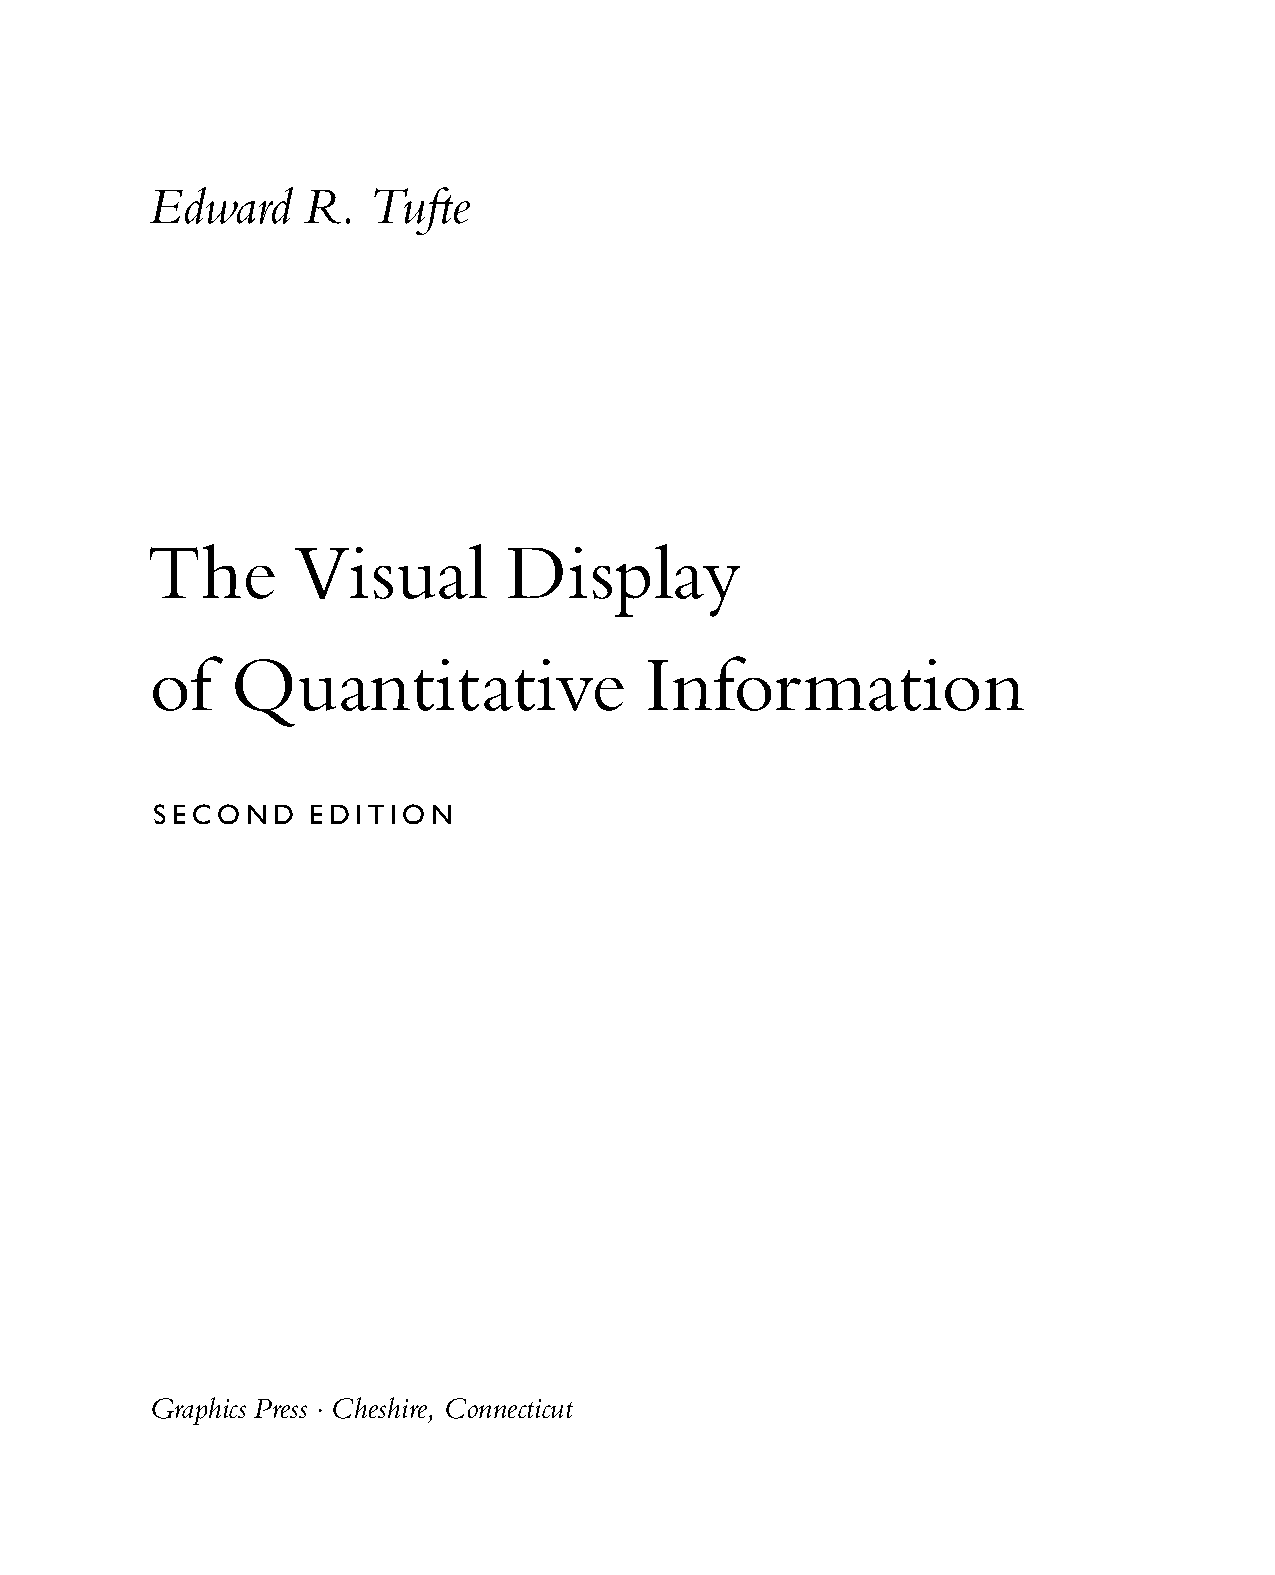
\includegraphics[width=0.45\linewidth]{vdqi-title.pdf}}
%\hfill
%\fbox{
\includegraphics[width=0.45\linewidth]{ei-title.pdf}}
%\\\vspace{\baselineskip}
%\fbox{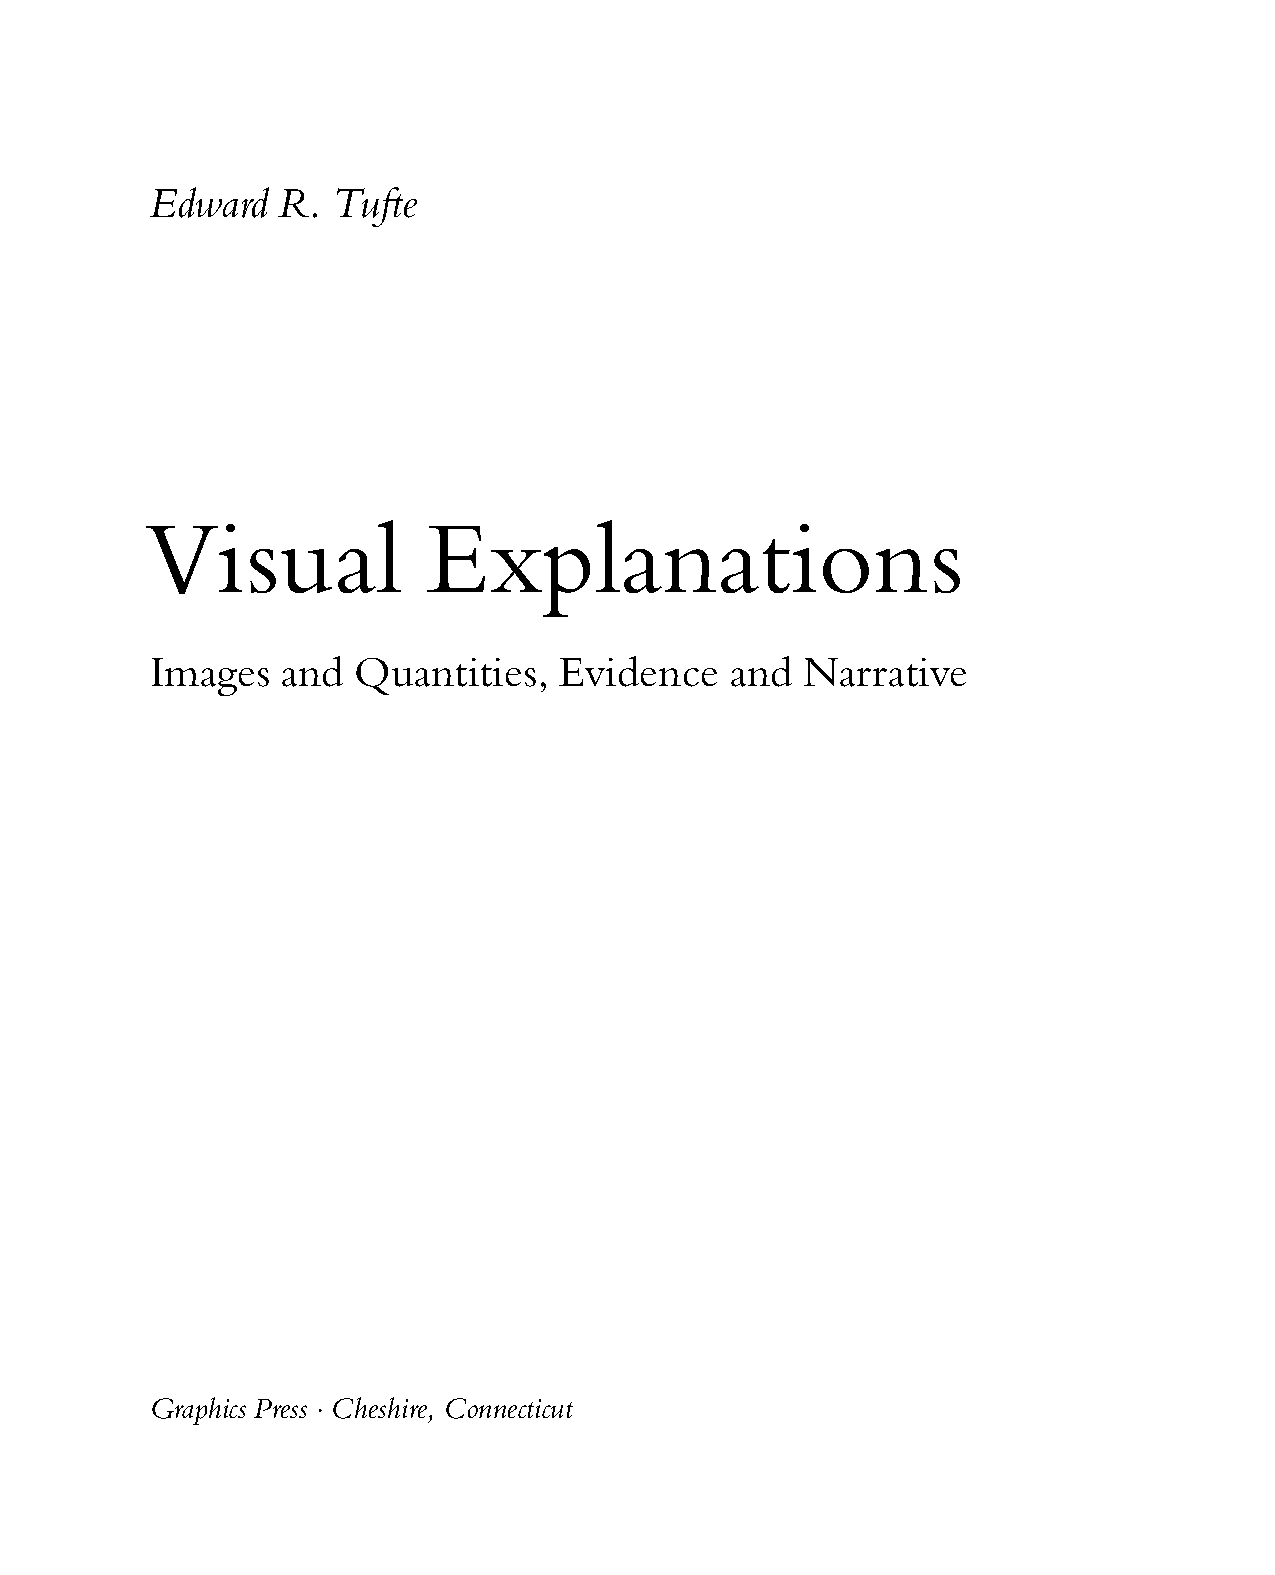
\includegraphics[width=0.45\linewidth]{ve-title.pdf}}
%\hfill
%\fbox{\includegraphics[width=0.45\linewidth]{be-title.pdf}}
%\end{figure*}
%

%\section{Headings}\label{sec:headings1}\index{headings}
%
%Tufte's books include the following heading levels: parts,
%chapters,\sidenote{Parts and chapters are defined for the \texttt{tufte-book}
%class only.}  sections, subsections, and paragraphs.  Not defined by default
%are: sub-subsections and subparagraphs.
%
%\begin{table}[h]
%  \begin{center}
%    \footnotesize%
%    \begin{tabular}{lcr}
%      \toprule
%      Heading & Style & Size \\
%      \midrule
%      Part & roman & \measure{24}{36}{40} \\
%      Chapter & italic & \measure{20}{30}{40} \\
%      Section & italic & \measure{12}{16}{26} \\
%      Subsection & italic & \measure{11}{15}{26} \\
%      Paragraph & italic & 10/14 \\
%      \bottomrule
%    \end{tabular}
%  \end{center}
%  \caption{Heading styles used in \BE.}
%  \label{tab:heading-styles}
%\end{table}
%
%\paragraph{Paragraph} Paragraph headings (as shown here) are introduced by
%italicized text and separated from the main paragraph by a bit of space.
%
%\section{Environments}
%
%The following characteristics define the various environments:
%
%
%\begin{table}[h]
%  \begin{center}
%    \footnotesize%
%    \begin{tabular}{lcl}
%      \toprule
%      Environment & Font size & Notes \\
%      \midrule
%      Body text & \measure{10}{14}{26} & \\
%      Block quote & \measure{9}{12}{24} & Block indent (left and right) by \unit[1]{pc} \\
%      Sidenotes & \measure{8}{10}{12} & Sidenote number is set inline, followed by word space \\
%      Captions & \measure{8}{10}{12} &  \\
%      \bottomrule
%    \end{tabular}
%  \end{center}
%  \caption{Environment styles used in \BE.}
%  \label{tab:environment-styles}
%\end{table}
%
%
%\chapter[On the Use of the tufte-book Document Class]{On the Use of the \texttt{tufte-book} Document Class}
%\label{ch:tufte-book}
%
%The \TL document classes define a style similar to the
%style Edward Tufte uses in his books and handouts.  Tufte's style is known
%for its extensive use of sidenotes, tight integration of graphics with
%text, and well-set typography.  This document aims to be at once a
%demonstration of the features of the \TL document classes
%and a style guide to their use.
%
%\section{Page Layout}\label{sec:page-layout}
%\subsection{Headings}\label{sec:headings}\index{headings}
%This style provides \textsc{a}- and \textsc{b}-heads (that is,
%\Verb|\section| and \Verb|\subsection|), demonstrated above.
%
%If you need more than two levels of section headings, you'll have to define
%them yourself at the moment; there are no pre-defined styles for anything below
%a \Verb|\subsection|.  As Bringhurst points out in \textit{The Elements of
%Typographic Style},\cite{Bringhurst2005} you should ``use as many levels of
%headings as you need: no more, and no fewer.''
%
%The \TL classes will emit an error if you try to use
%\linebreak\Verb|\subsubsection| and smaller headings.
%
%% let's start a new thought -- a new section
%\newthought{In his later books},\cite{Tufte2006} Tufte
%starts each section with a bit of vertical space, a non-indented paragraph,
%and sets the first few words of the sentence in \textsc{small caps}.  To
%accomplish this using this style, use the \doccmddef{newthought} command:
%\begin{docspec}
%  \doccmd{newthought}\{In his later books\}, Tufte starts\ldots
%\end{docspec}
%
%
%\section{Sidenotes}\label{sec:sidenotes}
%One of the most prominent and distinctive features of this style is the
%extensive use of sidenotes.  There is a wide margin to provide ample room
%for sidenotes and small figures.  Any \doccmd{footnote}s will automatically
%be converted to sidenotes.\footnote{This is a sidenote that was entered
%using the \texttt{\textbackslash footnote} command.}  If you'd like to place ancillary
%information in the margin without the sidenote mark (the superscript
%number), you can use the \doccmd{marginnote} command.\marginnote{This is a
%margin note.  Notice that there isn't a number preceding the note, and
%there is no number in the main text where this note was written.}
%
%The specification of the \doccmddef{sidenote} command is:
%\begin{docspec}
%  \doccmd{sidenote}[\docopt{number}][\docopt{offset}]\{\docarg{Sidenote text.}\}
%\end{docspec}
%
%Both the \docopt{number} and \docopt{offset} arguments are optional.  If you
%provide a \docopt{number} argument, then that number will be used as the
%sidenote number.  It will change of the number of the current sidenote only and
%will not affect the numbering sequence of subsequent sidenotes.
%
%Sometimes a sidenote may run over the top of other text or graphics in the
%margin space.  If this happens, you can adjust the vertical position of the
%sidenote by providing a dimension in the \docopt{offset} argument.  Some
%examples of valid dimensions are:
%\begin{docspec}
%  \ttfamily 1.0in \qquad 2.54cm \qquad 254mm \qquad 6\Verb|\baselineskip|
%\end{docspec}
%If the dimension is positive it will push the sidenote down the page; if the
%dimension is negative, it will move the sidenote up the page.
%
%While both the \docopt{number} and \docopt{offset} arguments are optional, they
%must be provided in order.  To adjust the vertical position of the sidenote
%while leaving the sidenote number alone, use the following syntax:
%\begin{docspec}
%  \doccmd{sidenote}[][\docopt{offset}]\{\docarg{Sidenote text.}\}
%\end{docspec}
%The empty brackets tell the \Verb|\sidenote| command to use the default
%sidenote number.
%
%If you \emph{only} want to change the sidenote number, however, you may
%completely omit the \docopt{offset} argument:
%\begin{docspec}
%  \doccmd{sidenote}[\docopt{number}]\{\docarg{Sidenote text.}\}
%\end{docspec}
%
%The \doccmddef{marginnote} command has a similar \docarg{offset} argument:
%\begin{docspec}
%  \doccmd{marginnote}[\docopt{offset}]\{\docarg{Margin note text.}\}
%\end{docspec}
%
%\section{References}
%References are placed alongside their citations as sidenotes,
%as well.  This can be accomplished using the normal \doccmddef{cite}
%command.\sidenote{The first paragraph of this document includes a citation.}
%
%The complete list of references may also be printed automatically by using
%the \doccmddef{bibliography} command.  (See the end of this document for an
%example.)  If you do not want to print a bibliography at the end of your
%document, use the \doccmddef{nobibliography} command in its place.  
%
%To enter multiple citations at one location,\cite[-3\baselineskip]{Tufte2006,Tufte1990} you can
%provide a list of keys separated by commas and the same optional vertical
%offset argument: \Verb|\cite{Tufte2006,Tufte1990}|.  
%\begin{docspec}
%  \doccmd{cite}[\docopt{offset}]\{\docarg{bibkey1,bibkey2,\ldots}\}
%\end{docspec}
%
%\section{Figures and Tables}\label{sec:figures-and-tables}
%Images and graphics play an integral role in Tufte's work.
%In addition to the standard \docenvdef{figure} and \docenvdef{tabular} environments,
%this style provides special figure and table environments for full-width
%floats.
%
%Full page--width figures and tables may be placed in \docenvdef{figure*} or
%\docenvdef{table*} environments.  To place figures or tables in the margin,
%use the \docenvdef{marginfigure} or \docenvdef{margintable} environments as follows
%(see figure~\ref{fig:marginfig}):
%
%\begin{marginfigure}%
%  \includegraphics[width=\linewidth]{helix}
%  \caption{This is a margin figure.  The helix is defined by 
%    $x = \cos(2\pi z)$, $y = \sin(2\pi z)$, and $z = [0, 2.7]$.  The figure was
%    drawn using Asymptote (\url{http://asymptote.sf.net/}).}
%  \label{fig:marginfig}
%\end{marginfigure}
%
%\begin{docspec}
%\textbackslash begin\{marginfigure\}\\
%  \qquad\textbackslash includegraphics\{helix\}\\
%  \qquad\textbackslash caption\{This is a margin figure.\}\\
%  \qquad\textbackslash label\{fig:marginfig\}\\
%\textbackslash end\{marginfigure\}\\
%\end{docspec}
%
%The \docenv{marginfigure} and \docenv{margintable} environments accept an optional parameter \docopt{offset} that adjusts the vertical position of the figure or table.  See the ``\nameref{sec:sidenotes}'' section above for examples.  The specifications are:
%\begin{docspec}
%  \textbackslash{begin\{marginfigure\}[\docopt{offset}]}\\
%  \qquad\ldots\\
%  \textbackslash{end\{marginfigure\}}\\
%  \mbox{}\\
%  \textbackslash{begin\{margintable\}[\docopt{offset}]}\\
%  \qquad\ldots\\
%  \textbackslash{end\{margintable\}}\\
%\end{docspec}
%
%Figure~\ref{fig:fullfig} is an example of the \docenv{figure*}
%environment and figure~\ref{fig:textfig} is an example of the normal
%\docenv{figure} environment.
%
%\begin{figure*}[h]
%  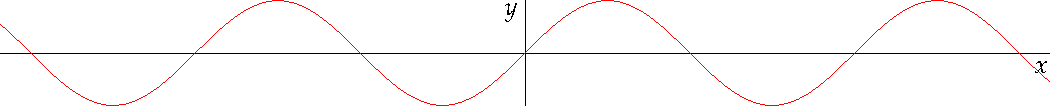
\includegraphics[width=\linewidth]{sine.pdf}%
%  \caption{This graph shows $y = \sin x$ from about $x = [-10, 10]$.
%  \emph{Notice that this figure takes up the full page width.}}%
%  \label{fig:fullfig}%
%\end{figure*}
%
%\begin{figure}
%  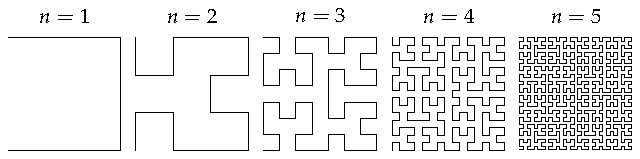
\includegraphics{hilbertcurves.pdf}
%%  \checkparity This is an \pageparity\ page.%
%  \caption[Hilbert curves of various degrees $n$.][6pt]{Hilbert curves of various degrees $n$. \emph{Notice that this figure only takes up the main textblock width.}}
%  \label{fig:textfig}
%  %\zsavepos{pos:textfig}
%\end{figure}
%
%As with sidenotes and marginnotes, a caption may sometimes require vertical
%adjustment. The \doccmddef{caption} command now takes a second optional
%argument that enables you to do this by providing a dimension \docopt{offset}.
%You may specify the caption in any one of the following forms:
%\begin{docspec}
%  \doccmd{caption}\{\docarg{long caption}\}\\
%  \doccmd{caption}[\docarg{short caption}]\{\docarg{long caption}\}\\
%  \doccmd{caption}[][\docopt{offset}]\{\docarg{long caption}\}\\
%  \doccmd{caption}[\docarg{short caption}][\docopt{offset}]%
%                  \{\docarg{long caption}\}
%\end{docspec}
%A positive \docopt{offset} will push the caption down the page. The short
%caption, if provided, is what appears in the list of figures/tables, otherwise
%the ``long'' caption appears there. Note that although the arguments
%\docopt{short caption} and \docopt{offset} are both optional, they must be
%provided in order. Thus, to specify an \docopt{offset} without specifying a
%\docopt{short caption}, you must include the first set of empty brackets
%\Verb|[]|, which tell \doccmd{caption} to use the default ``long'' caption. As
%an example, the caption to figure~\ref{fig:textfig} above was given in the form
%\begin{docspec}
%  \doccmd{caption}[Hilbert curves...][6pt]\{Hilbert curves...\}
%\end{docspec}
%
%Table~\ref{tab:normaltab} shows table created with the \docpkg{booktabs}
%package.  Notice the lack of vertical rules---they serve only to clutter
%the table's data.
%
%\begin{table}[ht]
%  \centering
%  \fontfamily{ppl}\selectfont
%  \begin{tabular}{ll}
%    \toprule
%    Margin & Length \\
%    \midrule
%    Paper width & \unit[8\nicefrac{1}{2}]{inches} \\
%    Paper height & \unit[11]{inches} \\
%    Textblock width & \unit[6\nicefrac{1}{2}]{inches} \\
%    Textblock/sidenote gutter & \unit[\nicefrac{3}{8}]{inches} \\
%    Sidenote width & \unit[2]{inches} \\
%    \bottomrule
%  \end{tabular}
%  \caption{Here are the dimensions of the various margins used in the Tufte-handout class.}
%  \label{tab:normaltab}
%  %\zsavepos{pos:normaltab}
%\end{table}
%
%\newthought{Occasionally} \LaTeX{} will generate an error message:\label{err:too-many-floats}
%\begin{docspec}
%  Error: Too many unprocessed floats
%\end{docspec}
%\LaTeX{} tries to place floats in the best position on the page.  Until it's
%finished composing the page, however, it won't know where those positions are.
%If you have a lot of floats on a page (including sidenotes, margin notes,
%figures, tables, etc.), \LaTeX{} may run out of ``slots'' to keep track of them
%and will generate the above error.
%
%\LaTeX{} initially allocates 18 slots for storing floats.  To work around this
%limitation, the \TL document classes provide a \doccmddef{morefloats} command
%that will reserve more slots.
%
%The first time \doccmd{morefloats} is called, it allocates an additional 34
%slots.  The second time \doccmd{morefloats} is called, it allocates another 26
%slots.
%
%The \doccmd{morefloats} command may only be used two times.  Calling it a
%third time will generate an error message.  (This is because we can't safely
%allocate many more floats or \LaTeX{} will run out of memory.)
%
%If, after using the \doccmd{morefloats} command twice, you continue to get the
%\texttt{Too many unprocessed floats} error, there are a couple things you can
%do.
%
%The \doccmddef{FloatBarrier} command will immediately process all the floats
%before typesetting more material.  Since \doccmd{FloatBarrier} will start a new
%paragraph, you should place this command at the beginning or end of a
%paragraph.
%
%The \doccmddef{clearpage} command will also process the floats before
%continuing, but instead of starting a new paragraph, it will start a new page.
%
%You can also try moving your floats around a bit: move a figure or table to the
%next page or reduce the number of sidenotes.  (Each sidenote actually uses
%\emph{two} slots.)
%
%After the floats have placed, \LaTeX{} will mark those slots as unused so they
%are available for the next page to be composed.
%
%\section{Captions}
%You may notice that the captions are sometimes misaligned.
%Due to the way \LaTeX's float mechanism works, we can't know for sure where it
%decided to put a float. Therefore, the \TL document classes provide commands to
%override the caption position.
%
%\paragraph{Vertical alignment} To override the vertical alignment, use the
%\doccmd{setfloatalignment} command inside the float environment.  For
%example:
%
%\begin{fullwidth}
%\begin{docspec}
%  \textbackslash begin\{figure\}[btp]\\
%  \qquad \textbackslash includegraphics\{sinewave\}\\
%  \qquad \textbackslash caption\{This is an example of a sine wave.\}\\
%  \qquad \textbackslash label\{fig:sinewave\}\\
%  \qquad \hlred{\textbackslash setfloatalignment\{b\}\% forces caption to be bottom-aligned}\\
%  \textbackslash end\{figure\}
%\end{docspec}
%\end{fullwidth}
%
%\noindent The syntax of the \doccmddef{setfloatalignment} command is:
%
%\begin{docspec}
%  \doccmd{setfloatalignment}\{\docopt{pos}\}
%\end{docspec}
%
%\noindent where \docopt{pos} can be either \texttt{b} for bottom-aligned
%captions, or \texttt{t} for top-aligned captions.
%
%\paragraph{Horizontal alignment}\label{par:overriding-horizontal}
%To override the horizontal alignment, use either the \doccmd{forceversofloat}
%or the \doccmd{forcerectofloat} command inside of the float environment.  For
%example:
%
%\begin{fullwidth}
%\begin{docspec}
%  \textbackslash begin\{figure\}[btp]\\
%  \qquad \textbackslash includegraphics\{sinewave\}\\
%  \qquad \textbackslash caption\{This is an example of a sine wave.\}\\
%  \qquad \textbackslash label\{fig:sinewave\}\\
%  \qquad \hlred{\textbackslash forceversofloat\% forces caption to be set to the left of the float}\\
%  \textbackslash end\{figure\}
%\end{docspec}
%\end{fullwidth}
%
%The \doccmddef{forceversofloat} command causes the algorithm to assume the
%float has been placed on a verso page---that is, a page on the left side of a
%two-page spread.  Conversely, the \doccmddef{forcerectofloat} command causes
%the algorithm to assume the float has been placed on a recto page---that is, a
%page on the right side of a two-page spread.
%
%
%\section{Full-width text blocks}
%
%In addition to the new float types, there is a \docenvdef{fullwidth}
%environment that stretches across the main text block and the sidenotes
%area.
%
%\begin{Verbatim}
%\begin{fullwidth}
%Lorem ipsum dolor sit amet...
%\end{fullwidth}
%\end{Verbatim}
%
%\begin{fullwidth}
%\small\itshape\lipsum[1]
%\end{fullwidth}
%
%\section{Typography}\label{sec:typography}
%
%\subsection{Typefaces}\label{sec:typefaces}\index{typefaces}
%If the Palatino, \textsf{Helvetica}, and \texttt{Bera Mono} typefaces are installed, this style
%will use them automatically.  Otherwise, we'll fall back on the Computer Modern
%typefaces.
%
%\subsection{Letterspacing}\label{sec:letterspacing}
%This document class includes two new commands and some improvements on
%existing commands for letterspacing.
%
%When setting strings of \allcaps{ALL CAPS} or \smallcaps{small caps}, the
%letter\-spacing---that is, the spacing between the letters---should be
%increased slightly.\cite{Bringhurst2005}  The \doccmddef{allcaps} command has proper letterspacing for
%strings of \allcaps{FULL CAPITAL LETTERS}, and the \doccmddef{smallcaps} command
%has letterspacing for \smallcaps{small capital letters}.  These commands
%will also automatically convert the case of the text to upper- or
%lowercase, respectively.
%
%The \doccmddef{textsc} command has also been redefined to include
%letterspacing.  The case of the \doccmd{textsc} argument is left as is,
%however.  This allows one to use both uppercase and lowercase letters:
%\textsc{The Initial Letters Of The Words In This Sentence Are Capitalized.}
%
%
%
%\section{Document Class Options}\label{sec:options}
%
%\index{class options|(}
%The \doccls{tufte-book} class is based on the \LaTeX\ \doccls{book}
%document class.  Therefore, you can pass any of the typical book
%options.  There are a few options that are specific to the
%\doccls{tufte-book} document class, however.
%
%The \docclsoptdef{a4paper} option will set the paper size to \smallcaps{A4} instead of
%the default \smallcaps{US} letter size.
%
%The \docclsoptdef{sfsidenotes} option will set the sidenotes and title block in a 
%\textsf{sans serif} typeface instead of the default roman.
%
%The \docclsoptdef{twoside} option will modify the running heads so that the page
%number is printed on the outside edge (as opposed to always printing the page
%number on the right-side edge in \docclsoptdef{oneside} mode).  
%
%The \docclsoptdef{symmetric} option typesets the sidenotes on the outside edge of
%the page.  This is how books are traditionally printed, but is contrary to
%Tufte's book design which sets the sidenotes on the right side of the page.
%This option implicitly sets the \docclsopt{twoside} option.
%
%The \docclsoptdef{justified} option sets all the text fully justified (flush left
%and right).  The default is to set the text ragged right.  
%The body text of Tufte's books are set ragged right.  This prevents
%needless hyphenation and makes it easier to read the text in the slightly
%narrower column.
%
%The \docclsoptdef{bidi} option loads the \docpkg{bidi} package which is used with
%\tXeLaTeX\ to typeset bi-directional text.  Since the \docpkg{bidi}
%package needs to be loaded before the sidenotes and cite commands are defined,
%it can't be loaded in the document preamble.
%
%The \docclsoptdef{debug} option causes the \TL classes to output debug
%information to the log file which is useful in troubleshooting bugs.  It will
%also cause the graphics to be replaced by outlines.
%
%The \docclsoptdef{nofonts} option prevents the \TL classes from
%automatically loading the Palatino and Helvetica typefaces.  You should use
%this option if you wish to load your own fonts.  If you're using \tXeLaTeX, this
%option is implied (\ie, the Palatino and Helvetica fonts aren't loaded if you
%use \tXeLaTeX).  
%
%The \docclsoptdef{nols} option inhibits the letterspacing code.  The \TL\
%classes try to load the appropriate letterspacing package (either pdf\TeX's
%\docpkg{letterspace} package or the \docpkg{soul} package).  If you're using
%\tXeLaTeX\ with \docpkg{fontenc}, however, you should configure your own
%letterspacing.  
%
%The \docclsoptdef{notitlepage} option causes \doccmd{maketitle} to generate a title
%block instead of a title page.  The \doccls{book} class defaults to a title
%page and the \doccls{handout} class defaults to the title block.  There is an
%analogous \docclsoptdef{titlepage} option that forces \doccmd{maketitle} to
%generate a full title page instead of the title block.
%
%The \docclsoptdef{notoc} option suppresses \TL's custom table of contents
%(\textsc{toc}) design.  The current \textsc{toc} design only shows unnumbered
%chapter titles; it doesn't show sections or subsections.  The \docclsopt{notoc}
%option will revert to \LaTeX's \textsc{toc} design.
%
%The \docclsoptdef{nohyper} option prevents the \docpkg{hyperref} package from
%being loaded.  The default is to load the \docpkg{hyperref} package and use the
%\doccmd{title} and \doccmd{author} contents as metadata for the generated
%\textsc{pdf}.
%
%\index{class options|)}
%
%
%
%\chapter[Customizing Tufte-LaTeX]{Customizing \TL}
%\label{ch:customizing}
%
%The \TL document classes are designed to closely emulate Tufte's book
%design by default.  However, each document is different and you may encounter
%situations where the default settings are insufficient.  This chapter explores
%many of the ways you can adjust the \TL document classes to better fit
%your needs.
%
%\section{File Hooks}
%\label{sec:filehooks}
%
%\index{file hooks|(}
%If you create many documents using the \TL classes, it's easier to
%store your customizations in a separate file instead of copying them into the
%preamble of each document.  The \TL classes provide three file hooks:
%\docfilehook{tufte-common-local.tex}{common}, \docfilehook{tufte-book-local.tex}{book}, and
%\docfilehook{tufte-handout-local.tex}{handout}.\sloppy
%
%\begin{description}
%  \item[\docfilehook{tufte-common-local.tex}{common}]
%    If this file exists, it will be loaded by all of the \TL document
%    classes just prior to any document-class-specific code.  If your
%    customizations or code should be included in both the book and handout
%    classes, use this file hook.
%  \item[\docfilehook{tufte-book-local.tex}{book}] 
%    If this file exists, it will be loaded after all of the common and
%    book-specific code has been read.  If your customizations apply only to the
%    book class, use this file hook.
%  \item[\docfilehook{tufte-common-handout.tex}{handout}] 
%    If this file exists, it will be loaded after all of the common and
%    handout-specific code has been read.  If your customizations apply only to
%    the handout class, use this file hook.
%\end{description}
%
%\index{file hooks|)}
%
%\section{Numbered Section Headings}
%\label{sec:numbered-sections}
%\index{headings!numbered}
%
%While Tufte dispenses with numbered headings in his books, if you require them,
%they can be anabled by changing the value of the \doccounter{secnumdepth}
%counter.  From the table below, select the heading level at which numbering
%should stop and set the \doccounter{secnumdepth} counter to that value.  For
%example, if you want parts and chapters numbered, but don't want numbering for
%sections or subsections, use the command:
%\begin{docspec}
%  \doccmd{ter}\{secnumdepth\}\{0\}
%\end{docspec}
%
%The default \doccounter{secnumdepth} for the \TL document classes is $-1$.
%
%\begin{table}
%  \footnotesize
%  \begin{center}
%    \begin{tabular}{lr}
%      \toprule
%      Heading level & Value \\
%      \midrule
%      Part (in \doccls{tufte-book}) & $-1$ \\
%      Part (in \doccls{tufte-handout}) & $0$ \\
%      Chapter (only in \doccls{tufte-book}) & $0$ \\
%      Section & $1$ \\
%      Subsection & $2$ \\
%      Subsubsection & $3$ \\
%      Paragraph & $4$ \\
%      Subparagraph & $5$ \\
%      \bottomrule
%    \end{tabular}
%  \end{center}
%  \caption{Heading levels used with the \texttt{secnumdepth} counter.}
%\end{table}
%
%\section{Changing the Paper Size}
%\label{sec:paper-size}
%
%The \TL classes currently only provide three paper sizes: \textsc{a4},
%\textsc{b5}, and \textsc{us} letter.  To specify a different paper size (and/or
%margins), use the \doccmd[geometry]{geometrysetup} command in the preamble of your
%document (or one of the file hooks).  The full documentation of the
%\doccmd{geometrysetup} command may be found in the \docpkg{geometry} package
%documentation.\cite{pkg-geometry}
%
%
%\section{Customizing Marginal Material}
%\label{sec:marginal-material}
%
%Marginal material includes sidenotes, citations, margin notes, and captions.
%Normally, the justification of the marginal material follows the justification
%of the body text.  If you specify the \docclsopt{justified} document class
%option, all of the margin material will be fully justified as well.  If you
%don't specify the \docclsopt{justified} option, then the marginal material will
%be set ragged right.
%
%You can set the justification of the marginal material separately from the body
%text using the following document class options: \docclsopt{sidenote},
%\docclsopt{marginnote}, \docclsopt{caption}, \docclsopt{citation}, and
%\docclsopt{marginals}.  Each option refers to its obviously corresponding
%marginal material type.  The \docclsopt{marginals} option simultaneously sets
%the justification on all four marginal material types.
%
%Each of the document class options takes one of five justification types:
%\begin{description}
%  \item[\docclsopt{justified}] Fully justifies the text (sets it flush left and
%    right).
%  \item[\docclsopt{raggedleft}] Sets the text ragged left, regardless of which
%    page it falls on.
%  \item[\docclsopt{raggedright}] Sets the text ragged right, regardless of
%    which page it falls on.
%  \item[\doccls{raggedouter}] Sets the text ragged left if it falls on the
%    left-hand (verso) page of the spread and otherwise sets it ragged right.
%    This is useful in conjunction with the \docclsopt{symmetric} document class
%    option.
%  \item[\docclsopt{auto}] If the \docclsopt{justified} document class option
%    was specified, then set the text fully justified; otherwise the text is set
%    ragged right.  This is the default justification option if one is not
%    explicitly specified.
%\end{description}
%
%\noindent For example, 
%\begin{docspec}
%  \doccmdnoindex{documentclass}[symmetric,justified,marginals=raggedouter]\{tufte-book\}
%\end{docspec}
%will set the body text of the document to be fully justified and all of the
%margin material (sidenotes, margin notes, captions, and citations) to be flush
%against the body text with ragged outer edges.
%
%\newthought{The font and style} of the marginal material may also be modified using the following commands:
%
%\begin{docspec}
%  \doccmd{setsidenotefont}\{\docopt{font commands}\}\\
%  \doccmd{setcaptionfont}\{\docopt{font commands}\}\\
%  \doccmd{setmarginnotefont}\{\docopt{font commands}\}\\
%  \doccmd{setcitationfont}\{\docopt{font commands}\}
%\end{docspec}
%
%The \doccmddef{setsidenotefont} sets the font and style for sidenotes, the
%\doccmddef{setcaptionfont} for captions, the \doccmddef{setmarginnotefont} for
%margin notes, and the \doccmddef{setcitationfont} for citations.  The
%\docopt{font commands} can contain font size changes (e.g.,
%\doccmdnoindex{footnotesize}, \doccmdnoindex{Huge}, etc.), font style changes (e.g.,
%\doccmdnoindex{sffamily}, \doccmdnoindex{ttfamily}, \doccmdnoindex{itshape}, etc.), color changes (e.g.,
%\doccmdnoindex{color}\texttt{\{blue\}}), and many other adjustments.
%
%If, for example, you wanted the captions to be set in italic sans serif, you could use:
%\begin{docspec}
%  \doccmd{setcaptionfont}\{\doccmdnoindex{itshape}\doccmdnoindex{sffamily}\}
%\end{docspec}
%
%\chapter{Compatibility Issues}
%\label{ch:compatibility}
%
%When switching an existing document from one document class to a \TL document class, a few changes to the document may have to be made.
%
%\section{Converting from \doccls{article} to \doccls{tufte-handout}}
%
%The following \doccls{article} class options are unsupported: \docclsopt{10pt}, \docclsopt{11pt}, \docclsopt{12pt}, \docclsopt{a5paper}, \docclsopt{b5paper}, \docclsopt{executivepaper}, \docclsopt{legalpaper}, \docclsopt{landscape}, \docclsopt{onecolumn}, and \doccls{twocolumn}.
%
%The following headings are not supported: \doccmd{subsubsection} and \doccmd{subparagraph}.
%
%\section{Converting from \doccls{book} to \doccls{tufte-book}}
%
%The following \doccls{report} class options are unsupported: \docclsopt{10pt}, \docclsopt{11pt}, \docclsopt{12pt}, \docclsopt{a5paper}, \docclsopt{b5paper}, \docclsopt{executivepaper}, \docclsopt{legalpaper}, \docclsopt{landscape}, \docclsopt{onecolumn}, and \doccls{twocolumn}.
%
%The following headings are not supported: \doccmd{subsubsection} and \doccmd{subparagraph}.
%
%
%
%\chapter{Troubleshooting and Support}
%\label{ch:troubleshooting}
%
%\section{\TL Website}\label{sec:website}
%The website for the \TL packages is located at
%\url{http://code.google.com/p/tufte-latex/}.  On our website, you'll find
%links to our \smallcaps{svn} repository, mailing lists, bug tracker, and documentation.
%
%\section{\TL Mailing Lists}\label{sec:mailing-lists}
%There are two mailing lists for the \TL project:
%
%\paragraph{Discussion list}
%The \texttt{tufte-latex} discussion list is for asking questions, getting
%assistance with problems, and help with troubleshooting.  Release announcements
%are also posted to this list.  You can subscribe to the \texttt{tufte-latex}
%discussion list at \url{http://groups.google.com/group/tufte-latex}.
%
%\paragraph{Commits list}
%The \texttt{tufte-latex-commits} list is a read-only mailing list.  A message
%is sent to the list any time the \TL code has been updated.  If you'd like to
%keep up with the latest code developments, you may subscribe to this list.  You
%can subscribe to the \texttt{tufte-latex-commits} mailing list at
%\url{http://groups.google.com/group/tufte-latex-commits}.
%
%\section{Getting Help}\label{sec:getting-help}
%If you've encountered a problem with one of the \TL document classes, have a
%question, or would like to report a bug, please send an email to our
%mailing list or visit our website.
%
%To help us troubleshoot the problem more quickly, please try to compile your
%document using the \docclsopt{debug} class option and send the generated
%\texttt{.log} file to the mailing list with a brief description of the problem.
%
%
%
%\section{Errors, Warnings, and Informational Messages}\label{sec:tl-messages}
%The following is a list of all of the errors, warnings, and other messages generated by the \TL classes and a brief description of their meanings.
%\index{error messages}\index{warning messages}\index{debug messages}
%
%% Errors
%\docmsg{Error: \doccmd{subparagraph} is undefined by this class.}{%
%The \doccmd{subparagraph} command is not defined in the \TL document classes.
%If you'd like to use the \doccmd{subparagraph} command, you'll need to redefine
%it yourself.  See the ``Headings'' section on page~\pageref{sec:headings} for a
%description of the heading styles availaboe in the \TL document classes.}
%
%\docmsg{Error: \doccmd{subsubsection} is undefined by this class.}{%
%The \doccmd{subsubsection} command is not defined in the \TL document classes.
%If you'd like to use the \doccmd{subsubsection} command, you'll need to
%redefine it yourself.  See the ``Headings'' section on
%page~\pageref{sec:headings} for a description of the heading styles availaboe
%in the \TL document classes.}
%
%\docmsg{Error: You may only call \doccmd{morefloats} twice. See the\par\noindent\ \ \ \ \ \ \ \ Tufte-LaTeX documentation for other workarounds.}{%
%\LaTeX{} allocates 18 slots for storing floats.  The first time
%\doccmd{morefloats} is called, it allocates an additional 34 slots.  The second
%time \doccmd{morefloats} is called, it allocates another 26 slots.
%
%The \doccmd{morefloats} command may only be called two times.  Calling it a
%third time will generate this error message.  See
%page~\pageref{err:too-many-floats} for more information.}
%
%% Warnings
%\docmsg{Warning: Option `\docopt{class option}' is not supported -{}- ignoring option.}{%
%This warning appears when you've tried to use \docopt{class option} with a \TL
%document class, but \docopt{class option} isn't supported by the \TL document
%class.  In this situation, \docopt{class option} is ignored.}
%
%% Info / Debug messages
%\docmsg{Info: The `\docclsopt{symmetric}' option implies `\docclsopt{twoside}'}{%
%You specified the \docclsopt{symmetric} document class option.  This option automatically forces the \docclsopt{twoside} option as well.  See page~\pageref{clsopt:symmetric} for more information on the \docclsopt{symmetric} class option.}
%
%
%\section{Package Dependencies}\label{sec:dependencies}
%The following is a list of packages that the \TL document
%classes rely upon.  Packages marked with an asterisk are optional.
%\begin{multicols}{2}
%\begin{itemize}
%  \item xifthen
%  \item ifpdf*
%  \item ifxetex*
%  \item hyperref
%  \item geometry
%  \item ragged2e
%  \item chngpage \emph{or} changepage
%  \item paralist
%  \item textcase
%  \item soul*
%  \item letterspace*
%  \item setspace
%  \item natbib \emph{and} bibentry
%  \item optparams
%  \item placeins
%  \item mathpazo*
%  \item helvet*
%  \item fontenc
%  \item beramono*
%  \item fancyhdr
%  \item xcolor
%  \item textcomp
%  \item titlesec
%  \item titletoc
%\end{itemize}
%\end{multicols}




%%
% The back matter contains appendices, bibliographies, indices, glossaries, etc.







\backmatter
\appendix
\chapter{Apéndice: Conceptos Matemáticos y de la Física Clásica
Importantes en Mecánica Cuántica}
\section{La Relación de Euler}
A menudo encontraremos en nuestras funciones de onda, términos
exponenciales imaginarios, como $\mathrm{e}^{\mathrm{i}\theta}$.
La relación de Euler (1707-1783), a la que Feynmann llamó "la
fórmula más sobresaliente de las matemáticas" permite expresar
este tipo de exponenciales a partir de funciones trigonométricas:
\begin{equation}
    \mathrm{e}^{\mathrm{i}\theta} = \cos{\theta} + \mathrm{i}\sin{\theta}
\end{equation}
Asímismo, para cualquier número imaginario $z=x + \mathrm{i}y$,
podemos escribir
\begin{equation}
    z=x + \mathrm{i}y = r(\cos{\theta} + \mathrm{i}\sin{\theta})=
    \mathrm{e}^{\mathrm{i}\theta}
\end{equation}
donde $\theta$ es el ángulo formado por la contribución 
real, $\mathrm{Re}(z)$, y la contribución imaginaria, 
$\mathrm{Im}(z)$, de $z$.





%\bibliography{sample-handout}
\bibliographystyle{plainnat}


%\printindex

\end{document}